\chapter{Descripción del Trabajo}
\label{cap:descripcionTrabajo}

En este capítulo se describiran los módulos que conforman la aplicación así como la arquitectura y las tecnologías utilizadas para su implementación.
\section{APRSINT}
La solución propuesta se ha llamado \textbf{APRSINT}, que es una combinación de los acrónimos APRS y OSINT. APRSINT está dividida en tres módulos principales:
\begin{itemize}
	\item \textbf{Adquisición de datos:} Este módulo se encargará de recopilar y almacenar los mensajes APRS de diversas fuentes, así como de integrar datos de otras fuentes abiertas y disponibles.
	\item \textbf{Procesamiento y análisis:} Este módulo se encargará de procesar y analizar los datos recopilados, ofreciendo herramientas avanzadas de visualización, filtrado y análisis de datos.
	\item \textbf{Visualización y presentación:} Este módulo se encargará de presentar los datos procesados y analizados de forma clara y comprensible, facilitando la interpretación y la toma de decisiones.
\end{itemize}

\begin{figure}[h]
    \centering
    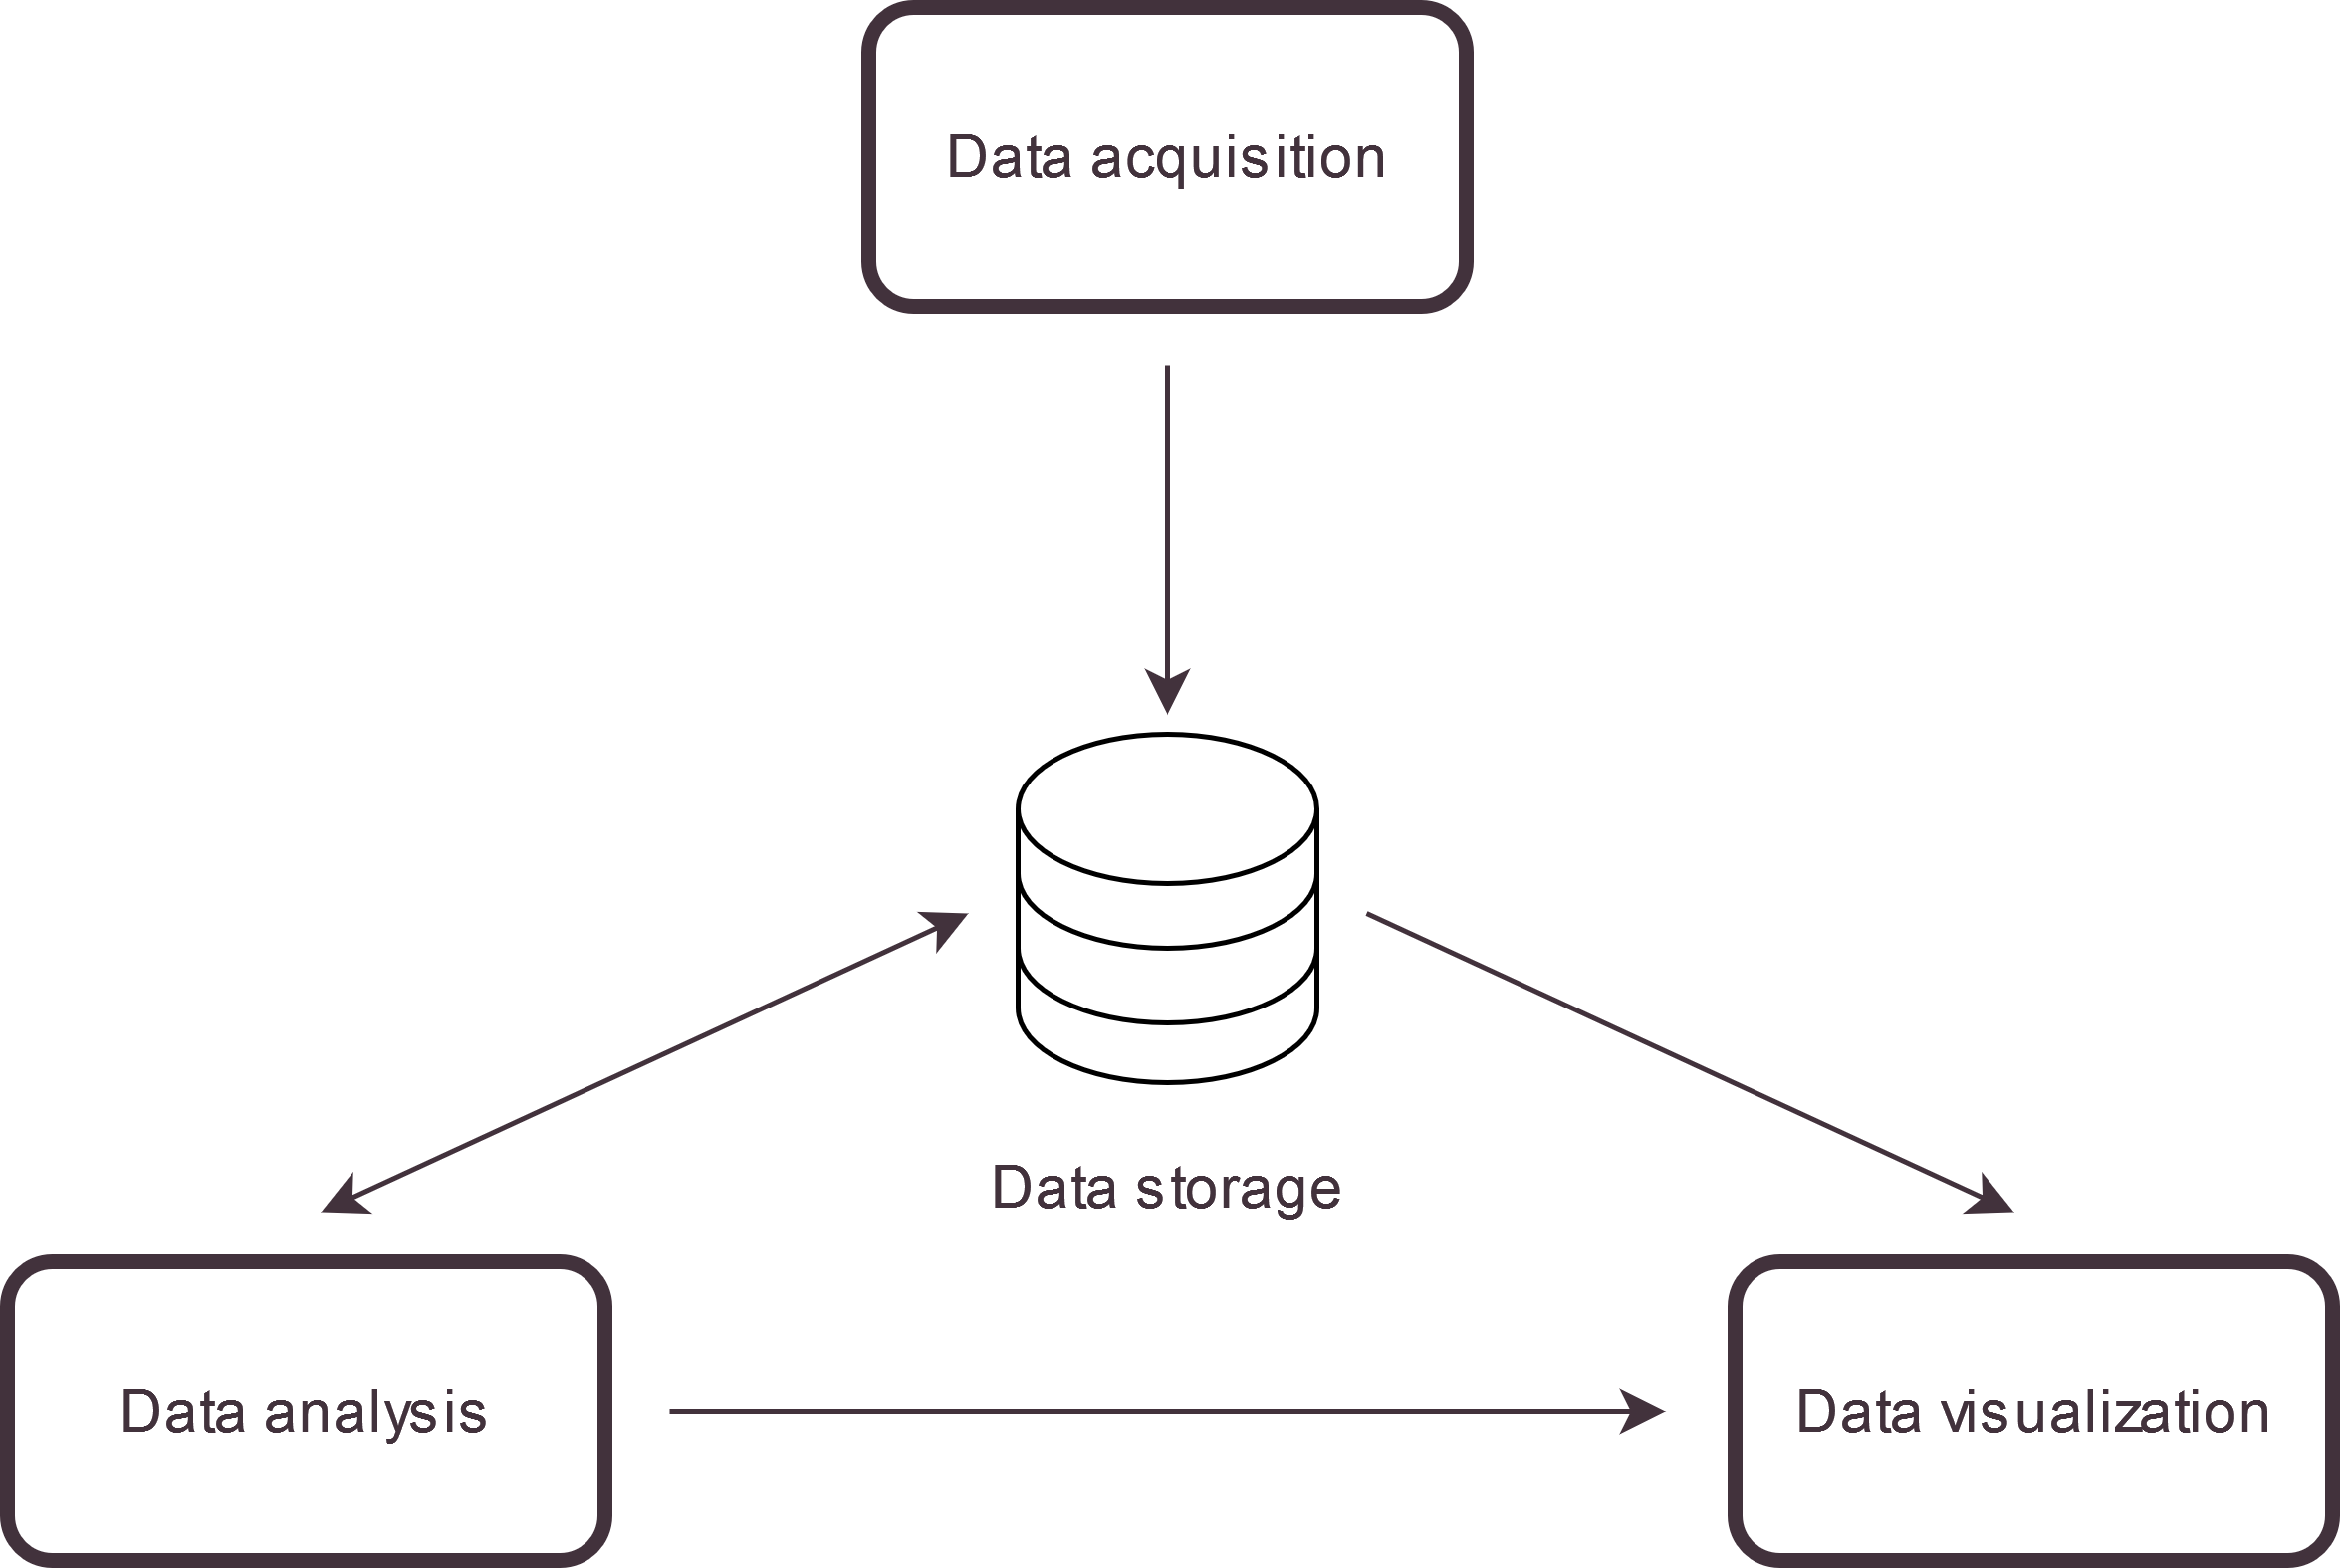
\includegraphics[width=0.65\textwidth]{Imagenes/Chapter_3/structure.png}
    \caption{Estructura base de la aplicación.}
    \label{fig:aprsint-logo}
\end{figure}

\section{Arquitectura de la aplicación}

Se pueden categorizar los tres módulos (\textbf{Adquisición de datos}, \textbf{Procesamiento y análisis}, \textbf{Visualización y presentación}) de la aplicación mencionados previamente en dos categorías principales:

\begin{itemize}
	\item \textbf{Adquisición de paquetes APRS:} En este módulo se encuentran los componentes encargados de la adquisición de paquetes APRS. Estos componentes se encargan de recibir los paquetes APRS, procesarlos y almacenarlos en la base de datos de la aplicación.

	\item \textbf{Aplicación web APRSINT:} En este módulo se encuentran los componentes encargados del análisis, la interpretación y la visualización, de los datos almacenados en la base de datos de la aplicación. Estos componentes se encargan de presentar la información de manera rápida y cómoda para el usuario.
\end{itemize}

\section{Tecnologías utilizadas (marco teórico)}

Como se ha mencionado anteriormente, uno de los objetivos de APRSINT es el de ser una solución accesible y fácil de usar. Para lograr este objetivo, se han seleccionado tecnologías ampliamente utilizadas y bien documentadas. A continuación se describen las tecnologías utilizadas en cada uno de los módulos de la aplicación.
\subsection{Raspberry Pi}

La Raspberry Pi es un \textit{Single board computer (SBC)} u ordenador de placa única desarrollada por la Fundación Raspberry Pi. Las Raspberry Pi son muy populares en el mundo de la informática y la electrónica por su bajo precio, reducido tamaño y su versatilidad.

\begin{itemize}
	\item \textbf{Bajo precio:} La Raspberry es una opción económica para implementar desde prototipos hasta aplicaciones simples, lo que la hace muy accesible para una amplia gama de usuarios.
	\item \textbf{Bajo consumo energético:} Su diseño de bajo consumo energético la hace ideal para aplicaciones que requieren funcionamiento continuo.
	\item \textbf{Versatilidad:} La Raspberry Pi 4 es altamente versátil y puede adaptarse a una variedad de casos de uso, desde servidores ligeros hasta placas de desarrollo para robótica y automatización.
\end{itemize}

\noindent Se ha seleccionado la Raspberry Pi 4B\footnote{Cuando se comenzó el proyecto todavía no se había lanzado la versión 5.} de 8GB de memoria RAM como plataforma de hardware para la implementación de la solución, debido a sus características y capacidades.

\subsection{Disco duro SSD}
Los discos duros de estado sólido (SSD) son una alternativa a los discos duros tradicionales (HDD) que ofrecen una mayor velocidad de lectura y escritura, menor consumo energético y mayor durabilidad. Se ha seleccionado un disco duro SSD de 250GB que se haya conectado a la Raspberry-pi para almacenar el gran volumen de datos que consume y genera la aplicación a su velocidad y fiabilidad.

\subsection{Python}
Python es un lenguaje de programación interpretado, de alto nivel y de propósito general. Es ampliamente utilizado en el desarrollo de aplicaciones web, científicas y de análisis de datos debido a su simplicidad, flexibilidad y facilidad de uso. Se ha seleccionado Python como lenguaje de programación principal para la implementación de la solución debido a la gran versatilidad que ofrece y sobre todo por la existencia de extensas librerías de visualización y manejo de grandes volúmenes de datos.

\subsection{Dash}
Dash es un \textit{framework} creado por Plotly que permite crear dashboards, aplicaciones web interactivas y visualizaciones de datos atractivas utilizando Python como lenguaje de programación. Se ha seleccionado Dash como \textit{framework} para la implementación de la interfaz web de la aplicación debido a su facilidad de uso y a la gran cantidad de funcionalidades que ofrece. Dash está escrito encima de Plotly.js, React y Flask lo que permite una gran capacidad de personalización.

\begin{itemize}
	\item \textbf{Interactividad:} Dash permite crear aplicaciones web altamente interactivas, lo que facilita la exploración de datos y la toma de decisiones.
	\item \textbf{Flexibilidad:} Su arquitectura modular y su amplia gama de componentes permiten la creación de aplicaciones web personalizadas y adaptadas a las necesidades específicas del usuario.
	\item \textbf{Integración con Plotly:} Al estar desarrollado por Plotly, Dash ofrece una integración perfecta con las capacidades de visualización de datos de Plotly, lo que permite crear gráficos y visualizaciones muy atractivas.
\end{itemize}

\noindent Para crear la aplicación web se consideraron algunas alternativas como Django, Streamlit y PowerBI, sin embargo, Dash fue la opción escogida debido a su extensa capacidad de personalización y personalización de la que carecían las demás opciones.

\subsection{Cosmograph JS}

Cosmograph es una librería de JavaScript enfocada en la visualización de grandes grafos y redes complejas en aplicaciones web. Permite representar de manera interactiva relaciones entre entidades, facilitando la comprensión y el análisis de datos estructurados.

\begin{itemize}
	\item \textbf{Visualización de grafos:} Cosmograph ofrece herramientas avanzadas para la representación visual de grafos como lineas temporales, histogramas y búsquedas de nodos, una mayor comprensión y capacidad de análisis de la información.

	\item \textbf{Rendimiento:} Cosmograph a diferencia de otras librerías más populares como Sigma JS transfiere todos los cálculos de posiciones de los nodos y aristas así como la representación gráfica de este a la GPU. Esto permite la visualización de grafos con miles de nodos y aristas sin afectar el rendimiento de la aplicación.

	\item \textbf{Personalización:} Ofrece opciones de personalización para adaptar la apariencia y el comportamiento de los nodos y aristas según las necesidades específicas del usuario.

\end{itemize}

\noindent Después de una gran cantidad de pruebas y tras considerar muchas alternativas como Sigma-JS, CytoScape y networkx, se acabó eligiendo Cosmograph sobre todo por su rendimiento.

\subsection{PostgreSQL}

PostgreSQL es un sistema de gestión de bases de datos relacional de código abierto y potente, conocido por su fiabilidad, robustez y capacidad para manejar grandes volúmenes de datos. Ofrece una amplia gama de características avanzadas que lo hacen adecuado para aplicaciones web y científicas que requieren almacenamiento y manipulación de datos complejos

\begin{itemize}
	\item \textbf{Fiabilidad y robustez:} PostgreSQL es conocido por su alta fiabilidad y capacidad para manejar grandes cargas de trabajo sin disminuir el rendimiento.
	\item \textbf{Escalabilidad:} Es altamente escalable y puede manejar grandes volúmenes de datos y transacciones concurrentes sin problemas.
	\item \textbf{Funcionalidades avanzadas:} Ofrece una amplia gama de funcionalidades avanzadas, como soporte para transacciones ACID, vistas materializadas, procedimientos almacenados y Full Text Search (búsqueda indexada).
	\item \textbf{Almacenamiento de datos semiestructurados:} PostgreSQL es capaz de almacenar y manipular datos no estructurados como JSON de manera eficiente, lo que lo hace adecuado para aplicaciones que requieren almacenamiento de datos semiestructurados.
	\item \textbf{Rendimiento:} PostgreSQL ofrece un muy buen rendimiento, especialmente en entornos de alta concurrencia y cargas de trabajo intensivas.
\end{itemize}

\noindent La elección de PostgreSQL como sistema de gestión de bases de datos se debió a su robustez, facilidad de uso y a la gran cantidad de funcionalidades que ofrece.

\subsection{SQLAlchemy}
SQLAlchemy es una biblioteca de Python que facilita la interacción con bases de datos relacionales utilizando un enfoque orientado a objetos. Permite trabajar con diferentes motores de bases de datos, como PostgreSQL, MySQL, SQLite, entre otros, de una manera consistente y eficiente.

\begin{itemize}
	\item \textbf{Abstracción de la base de datos:} SQLAlchemy proporciona una capa de abstracción sobre la base de datos, lo que permite a los desarrolladores interactuar con la base de datos utilizando objetos de Python en lugar de consultas SQL directas.
	\item \textbf{Compatibilidad con múltiples motores:} Es compatible con una variedad de motores de bases de datos, lo que brinda flexibilidad para trabajar con diferentes sistemas de gestión de bases de datos según las necesidades del proyecto. En este caso se ha utilizado el motor Psycopg2 para la conexión con PostgreSQL.
	\item \textbf{ORM (mapeo objeto-relacional):} Ofrece un ORM potente y flexible que mapea objetos Python a tablas de bases de datos, facilitando el manejo de relaciones entre objetos y la persistencia de datos.
	\item \textbf{Seguridad:} SQLAlchemy proporciona herramientas para prevenir ataques de inyección SQL y otros problemas de seguridad comunes en el manejo de bases de datos.
\end{itemize}

\noindent La elección de SQLAlchemy se ha basado en su capacidad para mejorar el proceso de interacción con la base de datos. Proporciona una estrecha integración entre la base de datos y la aplicación, permitiendo una flexibilidad muy grande a la hora de hacer consultas o inserciones y sobre todo creando una capa de seguridad para evitar ataques.

\subsection{Aprslib}
Aprslib es una biblioteca de Python que facilita la interacción con el sistema APRS. Permite recibir y decodificar paquetes APRS, así como enviar paquetes APRS a través de la red APRS-IS.
\begin{itemize}
	\item \textbf{Recepción de paquetes:} Aprslib permite recibir paquetes APRS de la red APRS-IS de manera sencilla.
	\item \textbf{Decodificación de paquetes:} Facilita la decodificación de paquetes APRS, permitiendo extraer información útil como la posición, velocidad y rumbo de los objetos rastreados.
	\item \textbf{Envío de paquetes:} Aprslib permite enviar paquetes APRS a través de la red APRS-IS, lo que facilita la integración con el sistema APRS.
\end{itemize}
\noindent Se ha elegido la librería Aprslib por su facilidad de uso, su documentación y su capacidad para decodificar los paquetes APRS.

\subsection{AWS}
Amazon Web Services (AWS) es una plataforma de servicios en la nube ofrecida por Amazon. Proporciona servicios de infraestructura informática, almacenamiento, bases de datos, análisis e inteligencia artificial, entre otros.

\begin{itemize}
	\item \textbf{Fiabilidad:} La infraestructura global de AWS está diseñada para ser altamente disponible y resistente a fallos, lo que garantiza la continuidad del servicio y la seguridad de los datos.
	\item \textbf{Variedad de servicios:} AWS ofrece una amplia gama de servicios, desde almacenamiento y bases de datos hasta aprendizaje automático y análisis de datos, lo que permite a las empresas construir y desplegar una amplia variedad de aplicaciones y soluciones.
	\item \textbf{Flexibilidad:} AWS proporciona opciones flexibles de implementación, incluyendo la capacidad de utilizar infraestructura física, virtual o basada en contenedores, según las necesidades del proyecto.
	\item \textbf{Seguridad:} AWS cuenta con medidas de seguridad muy robustas para proteger los datos y las aplicaciones, incluyendo controles de acceso, cifrado de datos y protección contra amenazas.
\end{itemize}

\noindent La elección de AWS así como los detalles de la implementación en la nube se describirán en la siguiente sección.

\subsection{Supervisord}
Supervisord es un sistema de control de procesos para sistemas operativos tipo Unix, diseñado para iniciar, detener y gestionar procesos de manera sencilla y robusta. Permite supervisar y mantener en funcionamiento aplicaciones y servicios, reiniciándolos automáticamente en caso de fallos o reinicios del sistema.

\begin{itemize}
	\item \textbf{Gestión de procesos:} Supervisord facilita la gestión de procesos al permitir iniciar, detener, reiniciar y supervisar procesos de manera centralizada.
	\item \textbf{Monitorización:} Supervisord proporciona información detallada sobre el estado de los procesos, incluyendo registros de eventos y estadísticas de rendimiento.
	\item \textbf{Reinicio automático:} En caso de fallos, Supervisord puede reiniciar automáticamente los procesos afectados, minimizando el tiempo de inactividad y manteniendo la disponibilidad del servicio.
\end{itemize}

\noindent Se ha seleccionado Supervisord como gestor de procesos gracias a su facilidad, flexibilidad (permitiendo ejecutar \textit{scripts} de Python directamente) y robustez.

\subsection{Pandas}
Pandas es la librería de facto de Python para gestionar y analizar datos estructurados. Al estar construida sobre Numpy (escrito en C), ofrece un rendimiento considerablemente superior a la implementación manual de estructuras de datos. Además de posibilitar la lectura y escritura de datos en diversos formatos, facilita la manipulación, limpieza y visualización de datos, convirtiéndola en una herramienta fundamental para el análisis de datos en Python.

\subsection{Conda}
Conda es un gestor de paquetes, entornos y canales de código abierto que facilita la instalación y gestión de paquetes y dependencias en Python. Conda permite crear entornos virtuales aislados para proyectos específicos, lo que facilita la gestión de dependencias y la compatibilidad entre versiones de paquetes. Se ha seleccionado Conda como gestor de paquetes para la instalación de las librerías y dependencias necesarias para la aplicación.

\begin{itemize}
	\item \textbf{Gestión de paquetes:} Conda facilita la instalación, actualización y eliminación de paquetes de \textit{software}. Esta característica es particularmente útil cuando se trabaja en proyectos que requieren bibliotecas específicas con versiones concretas.

	\item \textbf{Entornos virtuales:} Conda permite la creación de entornos virtuales independientes para cada proyecto. Esto significa que pueden existir diferentes versiones de paquetes instaladas en diferentes entornos sin que entren en conflicto entre sí. Esto es especialmente útil cuando se necesita trabajar en proyectos con diferentes requisitos de dependencias.

	\item \textbf{Portabilidad y reproducibilidad:} Al utilizar Conda para gestionar las dependencias de los proyectos, se puede garantizar que otros puedan reproducir el entorno de desarrollo exactamente como estaba. Esto es fundamental para la colaboración en proyectos de \textit{software} y la investigación reproducible en ciencia de datos.

	\item \textbf{Flexibilidad:} Conda no se limita solo al ecosistema de Python. También puede gestionar paquetes de otros lenguajes de programación, como R, Java y C/C++. Esto lo convierte en una herramienta versátil para proyectos que involucran múltiples tecnologías.
\end{itemize}

Se ha seleccionado Conda como gestor de paquetes debido a su facilidad de uso, su robustez y la gran cantidad de paquetes y librerías disponibles en su repositorio.

\subsection{Click}
Click es una librería de Python que permite la creación de herramientas de línea de comandos de manera sencilla y eficiente. Click facilita la creación de interfaces de usuario basadas en texto, lo que permite a los usuarios interactuar con las aplicaciones a través de la terminal. Se muestra un ejemplo de uso de Click en la \Cref{fig:click-example}.

\begin{figure}[!h]
	\centering
	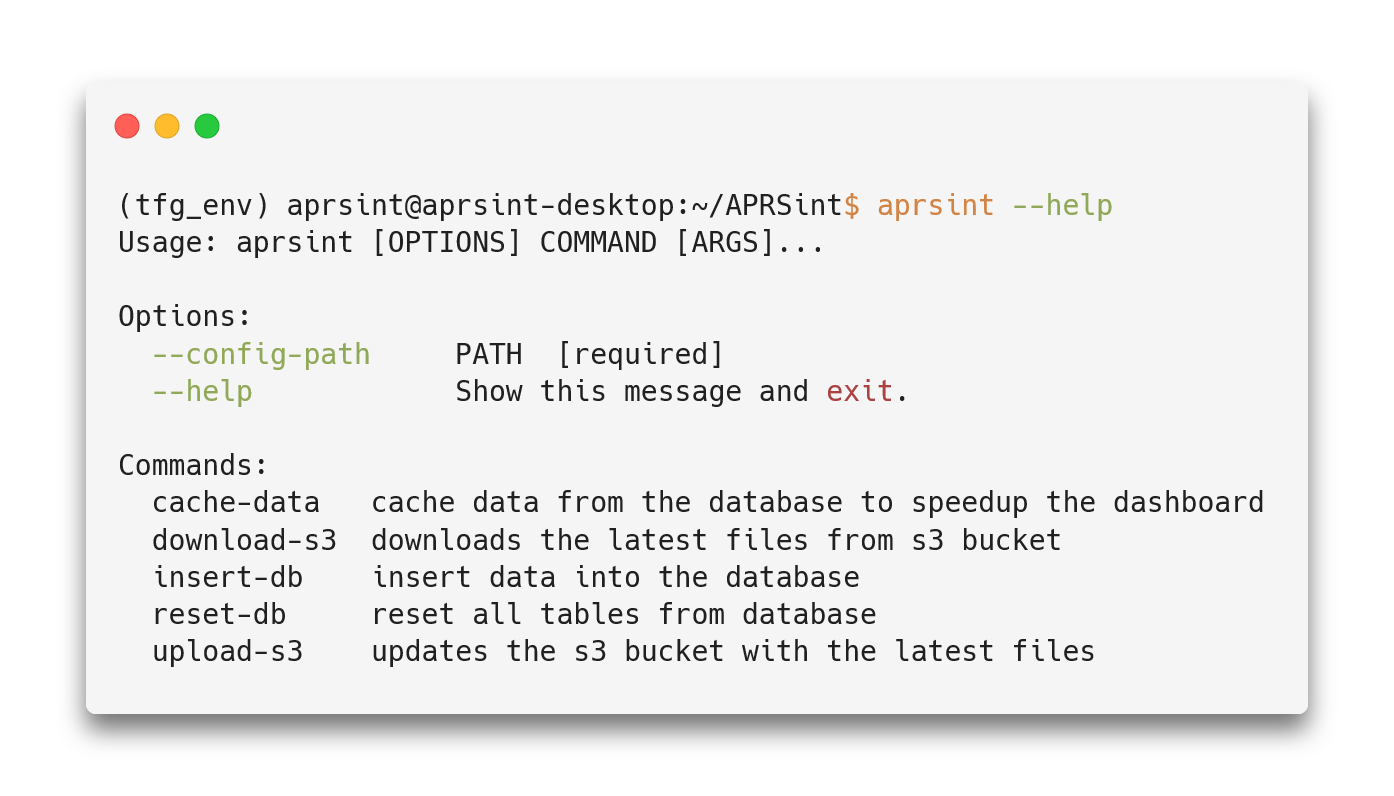
\includegraphics[width=0.85\textwidth]{Imagenes/Chapter_4/click_help.png}
	\caption[Ejemplo de uso de Click.]{Ejemplo de uso de Click (elaboración propia).}
	\label{fig:click-example}
\end{figure}

\subsection{Apache Airflow}
Apache Airflow es una plataforma de orquestación de tareas y flujos de trabajo. Es similar a Cron de Unix, pero permite una mayor personalización y control de las tareas que ejecuta. Las tareas se definen en archivos separados facilitando la compartimentalización y ofreciendo una mayor robustez y escalabilidad.
\begin{itemize}
	\item \textbf{Orquestación de flujos de trabajo:} Airflow facilita la orquestación de flujos de trabajo complejos al permitir definir tareas y sus dependencias como DAG's, lo que proporciona una visión clara de la lógica de ejecución.
	\item \textbf{Escalabilidad:} Airflow es altamente escalable y puede manejar flujos de trabajo de cualquier tamaño, desde tareas simples hasta flujos de trabajo altamente complejos.
	\item \textbf{Monitorización y alertas:} Proporciona una interfaz de usuario web para monitorizar el estado de los flujos de trabajo, así como capacidades de alerta para detectar y responder a fallos o retrasos en la ejecución de tareas.
	\item \textbf{Extensibilidad:} Airflow es altamente extensible y permite integrar fácilmente con otros sistemas y herramientas, lo que permite construir flujos de trabajo personalizados que se adapten a las necesidades específicas del proyecto.
\end{itemize}

\subsection{Configuración del proyecto}

Para la configuración del proyecto se ha utilizado un entorno virtual de Conda. Se ha creado un entorno virtual con las librerías necesarias para la ejecución de la aplicación. Algunas de las librerías más importantes que se han utilizado son las siguientes:

\begin{itemize}
	\item \textbf{Aprslib:} Para la recepción y decodificación de paquetes APRS.
	\item \textbf{Boto3:} Para la interacción con los servicios de AWS.
	\item \textbf{SQLAlchemy:} Para la interacción con la base de datos PostgreSQL.
	\item \textbf{Pandas:} Para la compresión y descompresión de ficheros.
	\item \textbf{Dash:} Para la creación de la aplicación web interactiva.
	\item \textbf{Click:} Para la creación de herramientas de línea de comandos.
\end{itemize}

Se ha creado un archivo de configuración en el que se definen las variables de entorno necesarias para la ejecución de la aplicación. Estas variables incluyen la configuración de la base de datos, las credenciales de AWS y la configuración de la aplicación web, entre otras.

Adicionalmente se ha configurado el proyecto con setuptools para facilitar la instalación y distribución de la aplicación. Se ha creado un archivo setup.py en el que se definen las dependencias del proyecto y se especifica la estructura del proyecto. Esto permite instalar la aplicación con un simple comando de pip.
$$pip\ install\ -i\ .$$

\section{Adquisición de datos}
En esta sección se describirá con detalle el módulo de adquisición de datos de la aplicación, incluyendo la arquitectura, los componentes y las tecnologías utilizadas.

\subsection{RTL-SDR}
En la primera fase del proyecto se adquirió un dongle RTL-SDR con el fin de recibir los paquetes APRS y procesarlos a partir de ello. Estos dongles son relativamente baratos oscilando entre los 30 y 100 euros, se conectan mediante usb al ordenador y disponen de un puerto SMA en la parte superior para la antena. La peculiaridad de estos dispositivos reside en que son controlables mediante \textit{software} y se pueden sintonizar en un rango de frecuencias muy amplio (24MHz a 1.7GHz).

Para utilizar estos dispositivos se necesita \textit{software} especializado como GQRX, CubicSDR o SDRSharp. Es posible también usar RTL-SDR en la terminal creando posteriormente un micrófono virtual para que el \textit{software} de análisis pueda decodificar los paquetes.

Tras multitud de pruebas fallidas con distintos \textit{software} de visualización y análisis y \textit{software} de audio como Direwolf, se decidió no continuar por ese camino y probar otras alternativas como la que finalmente se ha implementado y ha sido \textbf{APRS-IS}

\subsection{APRS-IS}
APRS-IS es un sistema que permite la transmisión de mensajes APRS por la red de Internet. La ventaja que ofrece este sistema frente al de recopilar información mediante una antena es que APRS-IS, permite obtener un flujo de datos mucho mayor, ya que hay una gran cantidad de antenas y otra ventaja con la que cuenta es que no está restringido al área que puede recibir la pequeña antena RTL-SDR sino a todo el mundo.

\subsubsection*{Infraestructura de la red APRS-IS}
Componentes principales:
\begin{itemize}
	\item \textbf{Trackers o TNC:} Son los emisores de los paquetes APRS, suelen corresponder a estaciones fijas o móviles que envían por radio los paquetes con información de posición, velocidad, rumbo, etc.
	\item \textbf{Digipeaters:} Son estaciones que reciben los paquetes APRS y los retransmiten, permitiendo que los paquetes lleguen a una mayor distancia. Son análogos a los repetidores de internet.
	\item \textbf{I-Gates:} Son estaciones que reciben los paquetes APRS por radio y los envían a la red APRS-IS, permitiendo que los paquetes sean accesibles a través de internet.
	\item \textbf{Servidores APRS-IS:} Son servidores que reciben los paquetes APRS de los I-Gates y los almacenan en una base de datos, permitiendo que los clientes accedan a los paquetes a través de internet. Los servidores APRS-IS suelen estar distribuidos geográficamente para mejorar la disponibilidad y la redundancia.
	\item \textbf{Clientes APRS-IS:} Pueden ser otros servidores, aplicaciones web o aplicaciones móviles que acceden a los servidores APRS-IS para obtener los paquetes APRS y mostrarlos a los usuarios.
\end{itemize}

La ruta que sigue un paquete APRS desde un tracker hasta un cliente APRS-IS se visualiza en la \Cref{fig:aprs-infra} y comprende los siguientes pasos: primero, un dispositivo \textbf{tracker} emite un paquete APRS a través de radiofrecuencia. Este paquete es recibido por un \textbf{Digipeater}, que funciona como un repetidor y retransmite la señal. Luego, un \textbf{I-Gate} recoge el paquete y lo envía a un servidor \textbf{APRS-IS} a través de Internet. Por último, un \textbf{cliente} APRS-IS accede a este servidor para recuperar el paquete y presentarlo al usuario para su visualización.

\begin{figure}[!h]
	\centering
	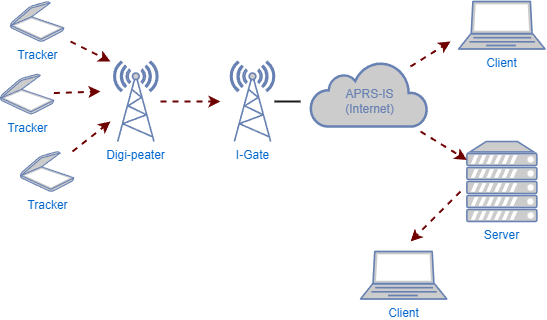
\includegraphics[width=0.95\textwidth]{Imagenes/Chapter_4/aprs_infra.png}
	\caption[Infraestructura de la red APRS - APRS-IS.]{Infraestructura de la red APRS - APRS-IS (elaboración propia).}
	\label{fig:aprs-infra}
\end{figure}

\FloatBarrier

Se ha seleccionado APRS-IS como fuente de datos para la aplicación debido a su facilidad de uso, su disponibilidad y la gran cantidad de información que ofrece desde sus servidores.

\subsection{La trama APRS}
El sistema APRS utiliza tramas AX.25 (Amateur X.25) para la transmisión de datos a través de las ondas de radio. El protocolo X.25 es un protocolo de nivel de enlace de datos que se diseñó y se creó para redes de conmutación de paquetes. El protocolo AX.25 es una versión simplificada del protocolo X.25 que se utiliza en las redes de radioaficionados.

\subsubsection*{Formato de la Trama APRS}

Todos los paquetes APRS se envían utilizando tramas \textbf{no numeradas} a diferencia de otros protocolos como TCP que utilizan tramas numeradas. Se muestra un ejemplo de trama APRS en la \Cref{fig:aprs-frame}.

\begin{figure}[h]
	\centering
	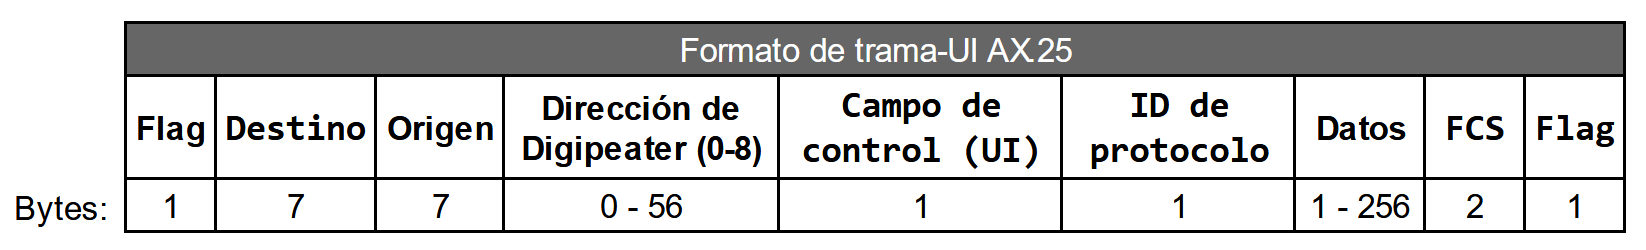
\includegraphics[width=1\textwidth]{Imagenes/Chapter_4/AX.25Frame.png}
	\caption[Formato de trama AX.25.]{Formato de trama AX.25 (elaboración propia, \cite{APRSProtocol}).}
	\label{fig:aprs-frame}
\end{figure}

Una trama AX.25 consta de los siguientes campos:
\begin{itemize}
	\item \textbf{Flag:} Marca el inicio y el final de la trama. Tiene un valor fijo de 0x7E.
	\item \textbf{Destino:} Identifica la estación de destino de la trama. Puede ser una dirección de estación completa o una dirección abreviada.
	\item \textbf{Origen:} Identifica la estación de origen de la trama. Puede ser una dirección de estación completa o una dirección abreviada.
	\item \textbf{Dirección de Digipeater (0-8):} Identifica los repetidores que deben reenviar la trama. Puede haber hasta 8 repetidores en la ruta.
	\item \textbf{Campo de control (UI):} Este campo se establece a 0x03 (trama no numerada).
	\item \textbf{ID de protocolo:} Este campo se establece a 0xF0 (no hay protocolo de capa 3).
	\item \textbf{Datos:} Este campo contiene los datos de la trama. En el caso de las tramas APRS, este campo puede contener información sobre la posición, la velocidad, el estado y otros datos de la estación.
	\item \textbf{FCS:} Frame Check Sequence (FCS): Es un código de verificación de redundancia cíclico (CRC) que se utiliza comprobar la integridad de la trama.
\end{itemize}


\subsubsection*{Contenido de la Trama}

Dentro del campo de información de una trama AX.25, se pueden incluir diversos datos relevantes para APRS. Esto puede incluir información de posición (latitud y longitud), velocidad, altitud, rumbo, comentarios del operador, mensajes de texto, etc ... \cite{APRSPaths}.

\[\underbrace{\textbf{\textcolor{red}{NOCALL}}}_{Origen}>\underbrace{\textbf{\textcolor[HTML]{FA9F42}{APRS}}}_{Destino}, \underbrace{\textbf{\textcolor{blue}{OH7RDA,OH7RDB}}}_{Digipeaters\ y\ I-Gates}:\underbrace{\textbf{\textcolor{green}{!4903N07201W-test A=001234}}}_{Campo\ datos}\]

En este ejemplo, el campo de datos contiene información sobre posición, altitud y un comentario. La posición está representada en formato APRS, que es una forma abreviada de representar la latitud y longitud en grados decimales. La altitud se representa en pies y el comentario es un mensaje de texto opcional, en este caso es ``test''.

\subsubsection*{Uso en APRS}

En el contexto de APRS, las tramas AX.25 se utilizan para transmitir actualizaciones de posición de estaciones móviles, estaciones meteorológicas, balizas y otros objetos de interés. Estas tramas son recibidas por otras estaciones en la red APRS, lo que permite el seguimiento en tiempo real de la ubicación y otros datos de interés.

\subsection{Recepción de paquetes APRS}

Para la recepción de paquetes APRS se ha utilizado la librería Aprslib de Python. Esta librería permite conectarse a un servidor APRS-IS y recibir los paquetes APRS en tiempo real. Se ha creado un sistema que utilizando esta librería se conecta a un servidor APRS-IS, recibe los paquetes APRS y los guarda en un \textit{buffer} en memoria. Cuando el \textit{buffer} se llena con aproximadamente 10.000 mensajes en alrededor de 15 segundos, se procede a escribir el \textit{buffer} en un fichero comprimido en el disco duro SSD.

Una detalle interesante es que los mensajes APRS no se decodifican en este punto, de hecho se guardan sin ningún tipo de procesamiento en ficheros binarios comprimidos en formato gzip para no ocupar mucho espacio en disco. Esto se hace así para evitar la sobrecarga de procesamiento en la Raspberry Pi y para poder procesar los mensajes en un servidor más potente en la nube.

Es importante mencionar que el sistema de recepción de paquetes APRS se ejecuta en segundo plano en modo demonio utilizando el gestor de procesos Supervisord, lo que garantiza que el sistema se mantenga en funcionamiento incluso en caso de fallos o reinicios del sistema.

\subsection{Procesado de paquetes APRS}
En esta sección se describirá con detalle el módulo de procesado de paquetes APRS de la aplicación, incluyendo la arquitectura, los componentes y las tecnologías utilizadas.

\subsubsection*{Subida de ficheros a AWS S3}

Una vez los ficheros se han guardado en el disco duro SSD, se procede a subirlos a un bucket S3 en AWS. Para ello se ha utilizado la librería Boto3 de Python, que permite interactuar con los servicios de AWS desde Python. Se ha creado un \textit{script} que se ejecuta una vez al día mediante la orquestación de Apache Airflow y que sube los ficheros comprimidos al bucket S3. Una vez subidos los ficheros, se eliminan del disco duro SSD para liberar espacio. Cuando un fichero se sube sube a S3 se desencadena un evento

\subsubsection*{Procesado de paquetes APRS en AWS Lambda}

Una vez los ficheros se han subido a S3, se desencadena un evento que ejecuta una función lambda \Cref{fig:aws-lambda} en AWS. Esta función lambda se encarga de descomprimir el fichero, procesar los mensajes APRS y convertirlos en formato JSON.

Por defecto Lambda no puede hacer uso de librerías de terceros por lo que se ha tenido que encapsular la librería Aprslib en un fichero .zip, subirlo a Lambda y establecerlo como una capa de Lambda para poder hacer uso de ella.

Para la descompresión de los ficheros se ha utilizado la librería gzip de Python, que permite leer y escribir ficheros comprimidos en formato gzip.
Para el procesado de los mensajes APRS se ha utilizado la librería Aprslib de Python como ya hemos mencionado, que permite decodificar los mensajes APRS y extraer información útil como la posición, velocidad y rumbo de los objetos rastreados en formato clave-valor.


\noindent Esta función lambda se ejecuta de manera asíncrona y paralela, lo que permite procesar grandes volúmenes de mensajes APRS de manera eficiente y escalable. Una vez procesados los mensajes APRS, se eliminan los ficheros comprimidos del S3 de entrada (aprsinput) para liberar espacio y evitar duplicados.

Finalmente los mensajes procesados se guardan en un bucket S3 de salida (aprsoutput) en formato JSON para su posterior descarga. La descarga de los ficheros JSON ocurre una vez al día mediante la orquestación de Apache Airflow y la librería Boto3. Estos ficheros (uno por fichero de entrada) se descargan a otra carpeta temporal en la Raspberry Pi.

\begin{figure}[h]
	\centering
	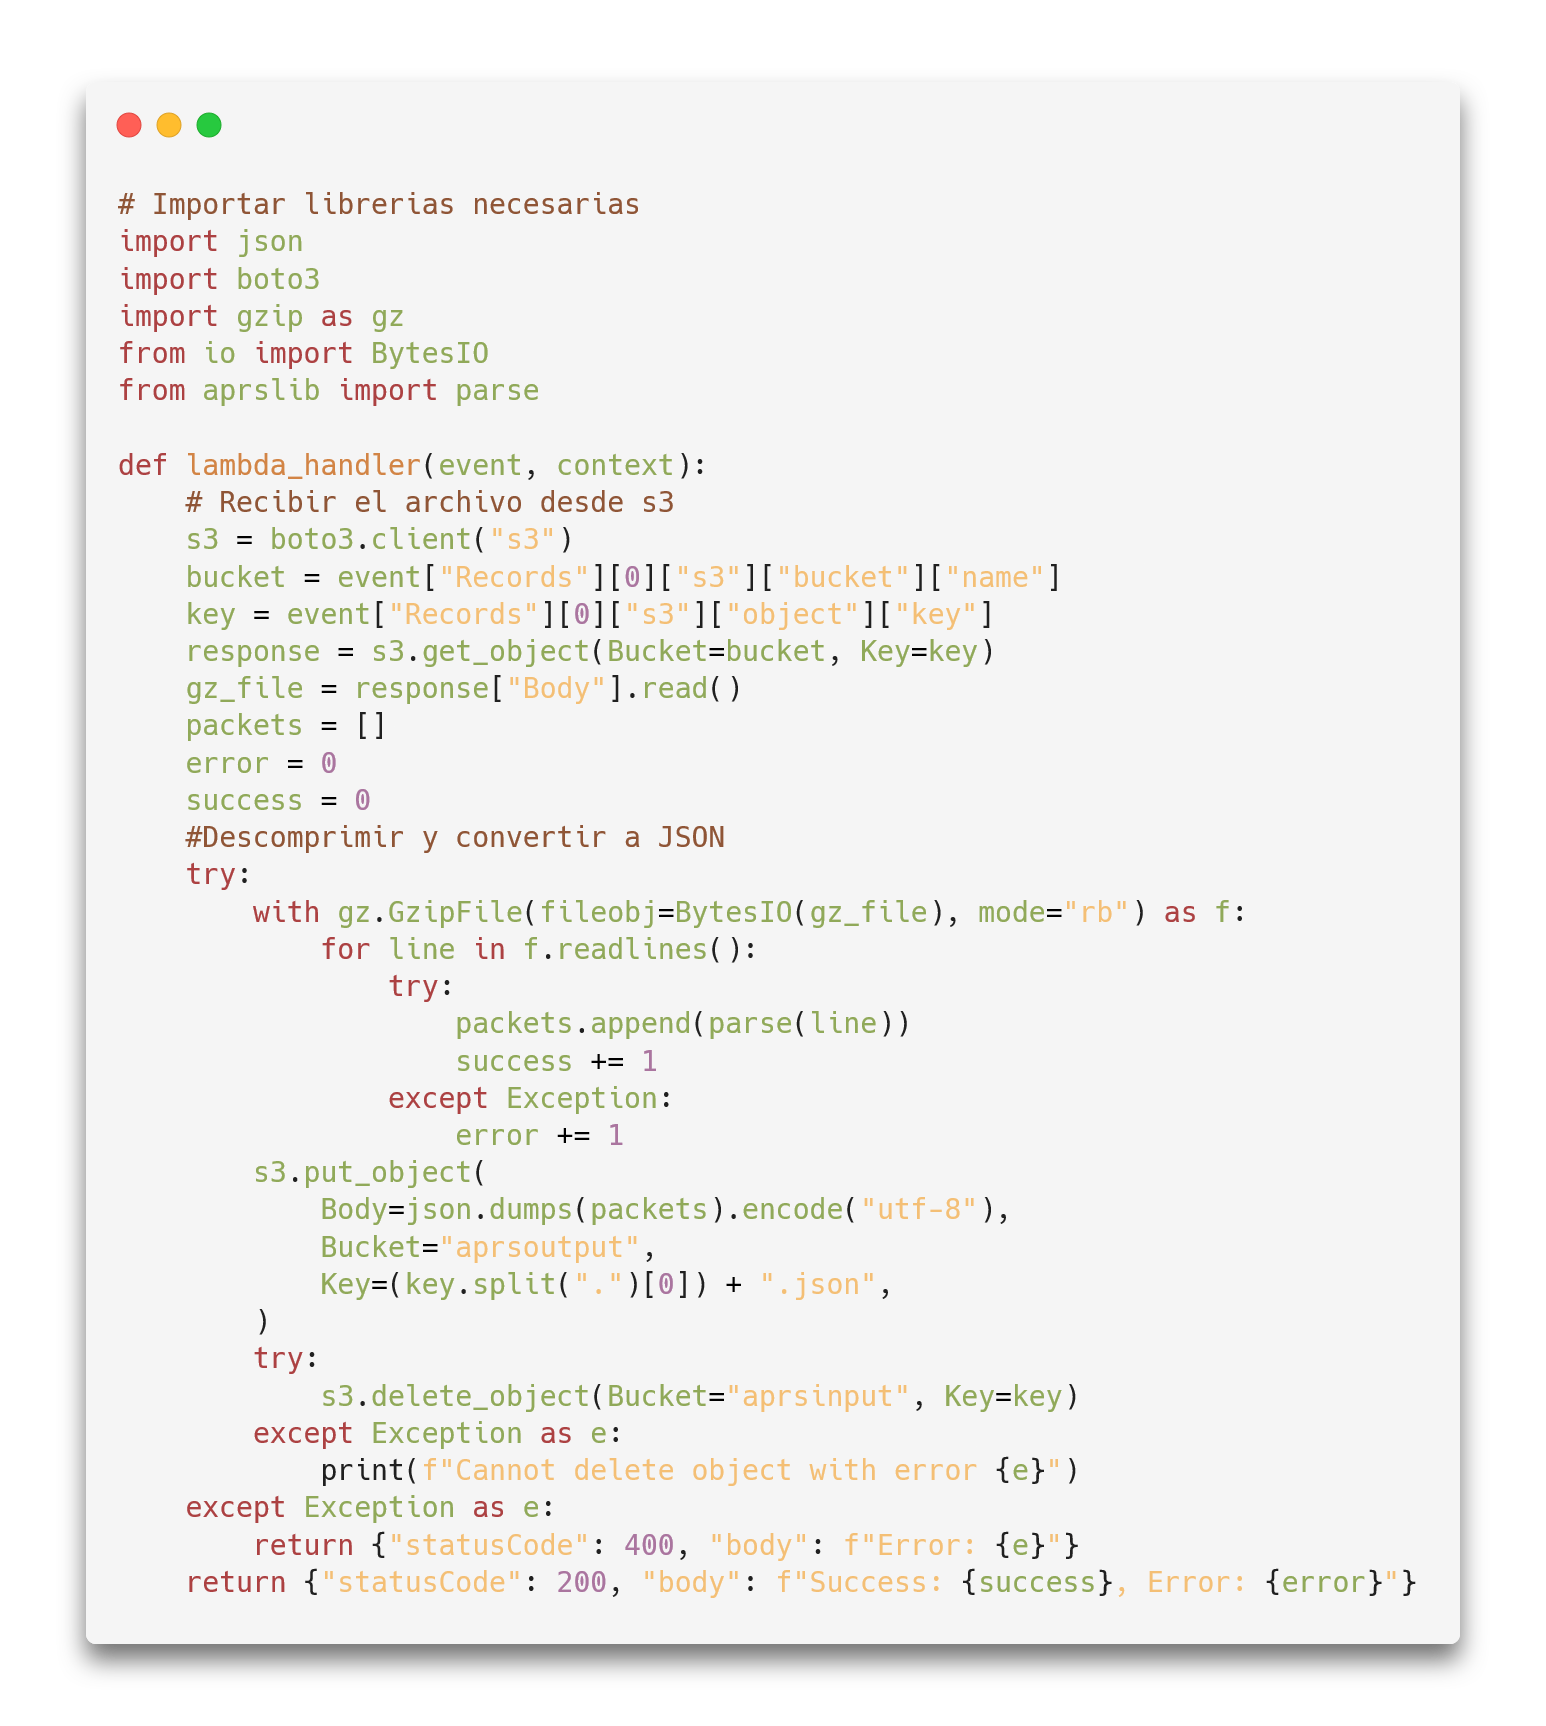
\includegraphics[width=0.8\textwidth]{Imagenes/Chapter_4/lambda.png}
	\caption[Procesado de paquetes APRS en AWS Lambda.]{Procesado de paquetes APRS en AWS Lambda (elaboración propia).}
	\label{fig:aws-lambda}
\end{figure}

\subsection{Almacenamiento de paquetes APRS en la base de datos}

Una vez los ficheros JSON ya procesados se han descargado al directorio temporal en la Raspberry Pi, se procede a almacenarlos en la base de datos PostgreSQL. Para ello se ha utilizado la librería SQLAlchemy de Python, que permite interactuar con bases de datos relacionales de manera sencilla y eficiente. Se ha creado un \textit{script} que se ejecuta una vez al día mediante la orquestación de Apache Airflow y que lee los ficheros JSON, procesa los mensajes APRS y los almacena en la base de datos.

Este paso esconde un gran problema que hubo de ser solucionado. El \textit{script} en un principio seguía los siguientes pasos.

\begin{enumerate}
	\item \textbf{Lectura de ficheros JSON:} El \textit{script} lee los ficheros JSON de la carpeta local /tmp descargados del bucket S3.
	\item \textbf{Extracción de la estación:} El \textit{script} extrae la estación origen y destino de cada mensaje y en caso de no existir en la base de datos las crea.
	\item \textbf{Extracción de las posiciones:} Se extraen las posiciones (si las hay) de cada mensaje y el timestamp si lo hay y se almacenan en la base de datos.
	\item \textbf{Identificación del país:} Mediante la librería Geopy y ficheros de formas de países se identifica el país de la estación.
	\item \textbf{Extracción de los mensajes:} Se extraen los mensajes de cada línea del JSON y se almacenan en la base de datos.
\end{enumerate}

\noindent Al utilizar este enfoque, se detectó un gran problema de rendimiento, ya que cada archivo JSON contenía alrededor de 10.000 mensajes y en la creación de los objetos, inserciones en la BD y detección del país se tardaba alrededor de 40 segundos por fichero JSON. Esto aunque no parezca demasiado tiempo, si se tiene en cuenta que la cantidad de mensajes APRS que se reciben en 40 segundos es alrededor de 45.000, se puede ver que el sistema no era escalable.

\subsubsection*{\underline{Optimizaciones}}
Para solucionar este problema se realizaron las siguientes optimizaciones:
\begin{itemize}
	\item \textbf{Uso de sets:} Se ha cambiado el uso de consultas a la BD por sets en la creación de las estaciones para acelerar la comprobación la existencia de una estación en la base de datos.
	\item \textbf{Inserción por lotes:} Se ha modificado la interfaz con SQLAlchemy para permitir inserciones en lotes de 250 mensajes.
	\item \textbf{Detección de países:} Se ha cambiado la librería Geopy por GeoPandas que permite la una detección de países más rápida utilizando paralelización.
\end{itemize}
Estas optimizaciones han acelerado el tiempo de procesado de un fichero JSON de 40 a 2 segundos, lo que ha permitido que el sistema sea escalable y pueda procesar grandes volúmenes de mensajes de manera eficiente.

\subsection{Base de datos}
Como se ha mencionado previamente, se ha elegido PostgreSQL como sistema de gestión de bases de datos para la aplicación. Esta elección se ha basado en la robustez, la fiabilidad y la capacidad de manejar grandes volúmenes de datos que ofrece PostgreSQL incluso en sistemas con recursos reducidos. La base de datos se ha diseñado siguiendo un modelo relacional \Cref{fig:db-model} que permite almacenar y relacionar la información de los mensajes APRS de manera eficiente, el modelo cuenta con las siguientes tablas.

\begin{itemize}
	\item \textbf{stations:} Almacena la información de las estaciones APRS, incluyendo el identificador de la estación (CALLSIGN), el ssid y su símbolo en formato caracter.
	\item \textbf{station\textunderscore locations:} Almacena la información de las posiciones \footnote[1]{Esta tabla tiene un campo id en la clave primaria por si una estación ha emitido un mensaje sin timestamp} de las estaciones APRS, incluyendo el país, la latitud, la longitud y la fecha y hora en la que se han recibido.
	\item \textbf{messages:} Almacena la información de los mensajes APRS, incluyendo el contenido del mensaje, el tipo de mensaje, el timestamp y el mensaje original retransmitido.
	\item \textbf{qrz\textunderscore profiles:} Sirve como una caché que almacena la información de los perfiles de los usuarios de QRZ, incluyendo el identificador (CALLSIGN), el nombre, la dirección, la ciudad, el estado, el código postal, el país, la latitud, la longitud y la fecha de nacimiento entre muchos otros.
\end{itemize}

\begin{figure}[h]
	\centering
	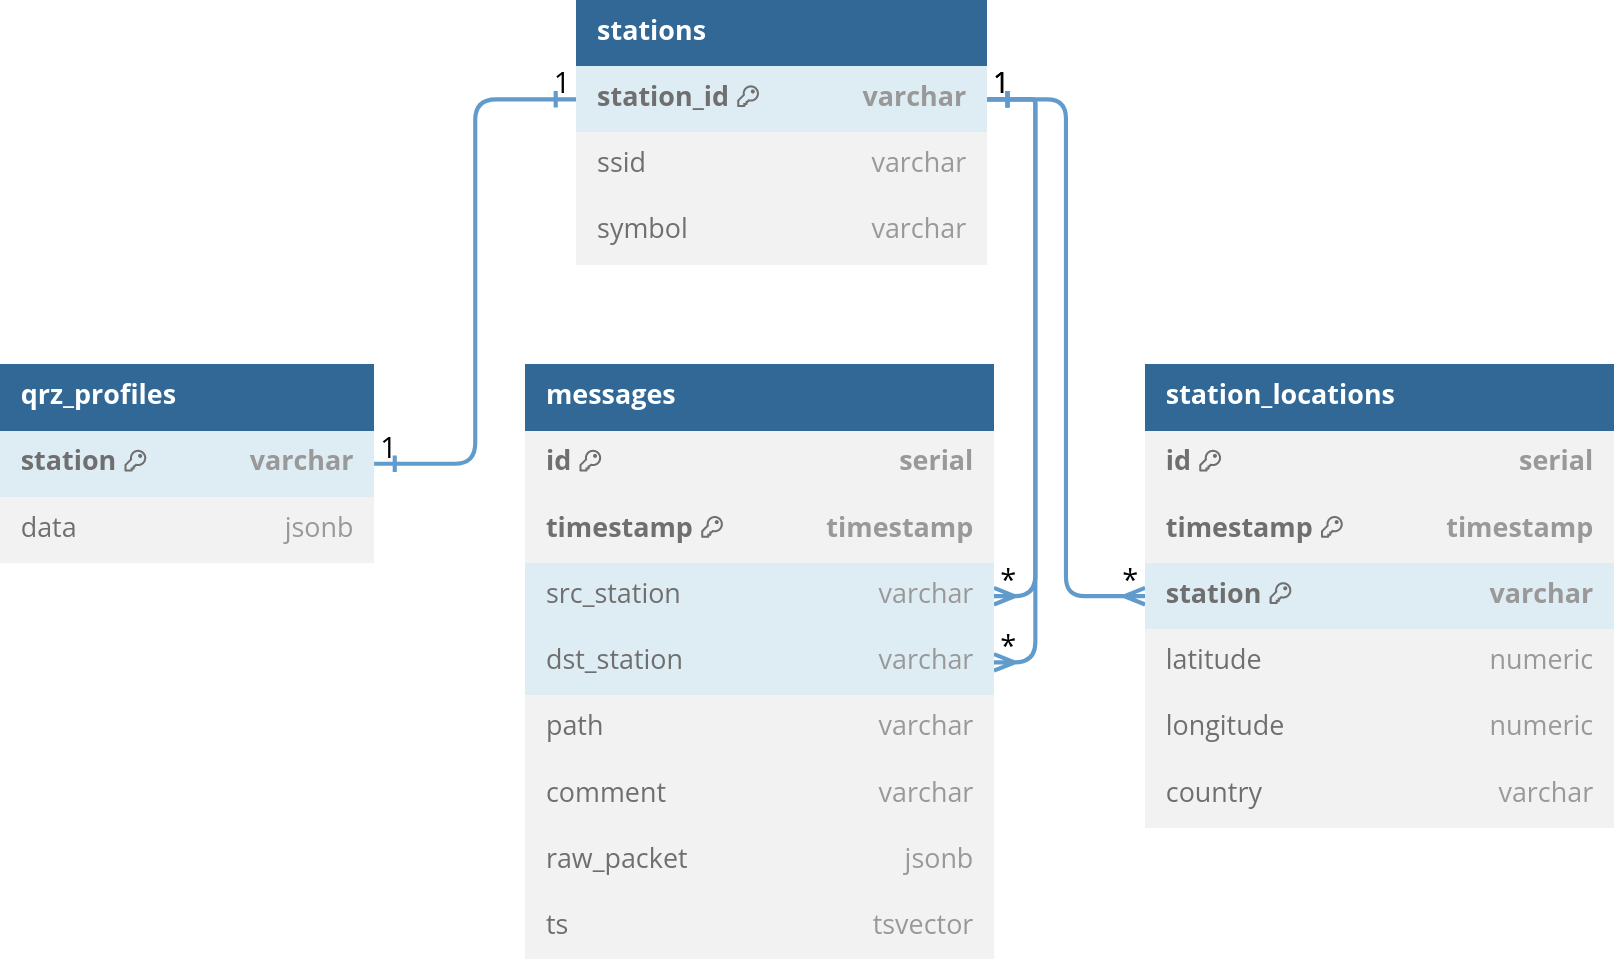
\includegraphics[width=0.9\textwidth]{Imagenes/Chapter_4/db_diagram.png}
	\caption[Estructura de la base de datos.]{Estructura de la base de datos (elaboración propia).}
	\label{fig:db-model}
\end{figure}

\FloatBarrier

\subsection{Flujo de un paquete APRS}
En esta sección se describe con detalle el flujo de un paquete APRS a través de la aplicación, desde la recepción hasta el almacenamiento en la base de datos.
\begin{enumerate}
	\item \textbf{Recepción:} El paquete APRS se recibe a través de la red APRS-IS y se almacena en un \textit{buffer} en memoria.
	\item \textbf{Almacenamiento en disco:} Cuando el \textit{buffer} se llena con aproximadamente 10.000 mensajes, se escribe el \textit{buffer} en un fichero comprimido en el disco duro SSD.
	\item \textbf{Subida a S3:} El fichero comprimido se sube a un bucket S3 en AWS para su procesamiento posterior.
	\item \textbf{Procesado en Lambda:} Una función lambda en AWS descomprime el fichero, procesa los mensajes APRS y los convierte en formato JSON.
	\item \textbf{Almacenamiento en S3:} Los ficheros JSON procesados se guardan en un bucket S3 de salida para su posterior descarga.
	\item \textbf{Descarga a la Raspberry Pi:} Una vez al día, los ficheros JSON se descargan a una carpeta temporal en la Raspberry Pi.
	\item \textbf{Almacenamiento en la base de datos:} Un \textit{script} en la Raspberry Pi lee los ficheros JSON, procesa los mensajes APRS y los almacena en la base de datos PostgreSQL.
\end{enumerate}


\section{Visualización y presentación de datos}

En esta sección se describe con detalle el módulo de visualización y presentación de datos de la aplicación, incluyendo la arquitectura, los componentes y las tecnologías utilizadas.

\subsection{Dash}
Dash es un \textit{framework} de Python creado por Plotly para la creación de aplicaciones web interactivas y visualizaciones de datos. Dash permite crear aplicaciones web interactivas y visualizaciones de datos atractivas utilizando Python como lenguaje de programación. Dash está escrito encima de Plotly.js, React y Flask lo que permite una gran capacidad de personalización.

Dash ofrece una versión de pago llamada Dash Enterprise que ofrece una gran cantidad de funcionalidades para elaborar aplicaciones web de manera más rápida y sencilla. Sin embargo, para este proyecto se ha utilizado la versión gratuita de Dash, con algunas librerías adicionales entre las que se encuentran:

\begin{itemize}
	\item \textbf{Dash core components:} Contiene multitud de componentes interactivos como gráficos, tablas, \textit{sliders}, \textit{dropdowns}, entre otros, que permiten a los usuarios interactuar con los datos de manera intuitiva.
	\item \textbf{Dash html components:} Contiene los \textit{wrappers} de las etiquetas HTML como \textit{divs}, \textit{spans}, \textit{inputs}, entre otros, que permiten personalizar la apariencia y el diseño de la aplicación web.
	\item \textbf{Dash mantine components:} Ofrece una amplia gama de componentes de Mantine como \textit{navbars}, tarjetas, modales, entre otros, que permiten crear aplicaciones web atractivas y responsivas.
	\item \textbf{Dash express:} Añade componentes extra como un panel de filtrado y una barra de navegación \footnote{Esta librería se ha modificado para adaptarla a las necesidades del proyecto.}.
	\item \textbf{Plotly express:} Es el principal competidor de Matplotlib en el mundo de la visualización de datos en Python. Ofrece una gran cantidad de gráficos y visualizaciones de datos interactivos.
\end{itemize}

\subsection{Diseño}
El diseño de la aplicación web se ha basado en la simplicidad, la usabilidad y la accesibilidad. El primer diseño del proyecto se realizó en la aplicación de prototipado Figma como se muestra en la \Cref{fig:figma}.

\begin{figure}[h]
	\centering
	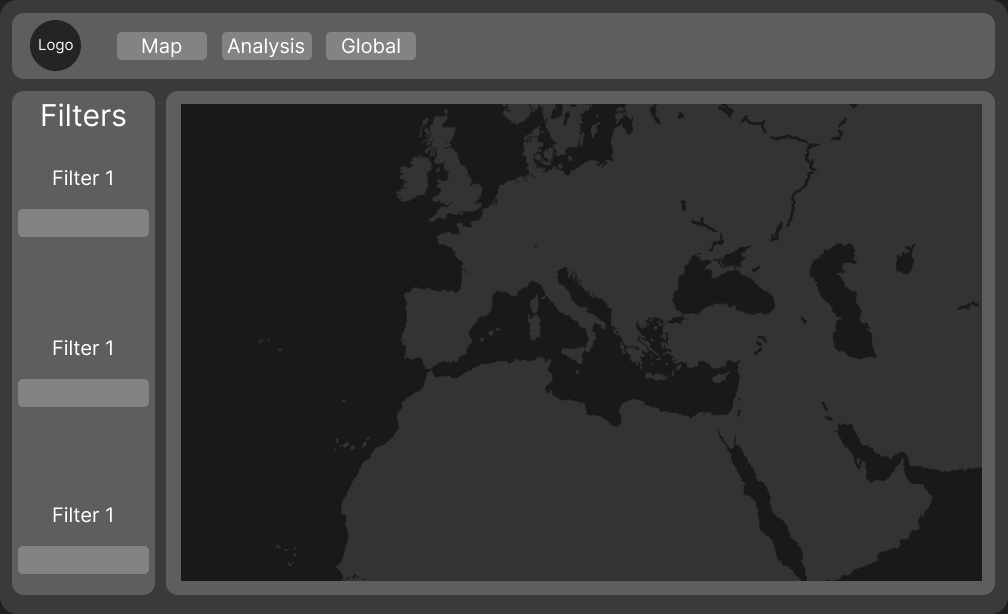
\includegraphics[width=0.8\textwidth]{Imagenes/Chapter_4/first_draft.png}
	\caption[Primer diseño de la aplicación web en Figma.]{Primer diseño de la aplicación web en Figma (elaboración propia).}
	\label{fig:figma}
\end{figure}

\noindent Este diseño se ha ido modificando y adaptando a lo largo del desarrollo del proyecto para mejorar la usabilidad y la experiencia del usuario. Este diseño muestra la pantalla principal de la aplicación, que incluye un mapa con las estaciones APRS, y un panel de control con filtros y opciones de visualización.

\subsection{Home - Primera pantalla}
En esta sección se describe la primera pantalla de la aplicación web, que muestra un mapa con las estaciones APRS y un panel de control con filtros y opciones de visualización.

\subsubsection*{Obtención de datos}

Siguiendo la estrategia de otros sistemas de \textit{dashboarding} como PowerBI o Tableau y con el objetivo de mejorar la eficiencia y la escalabilidad del sistema, se ha optado por eliminar en lo posible las consultas a la base de datos en tiempo real. Para ello se ha creado un sistema de caché que almacena los datos a representar en esta pantalla en un archivo de rápida lectura que es actualizado diariamente mediante Apache Airflow. Este sistema de caché permite reducir la carga en la base de datos y mejorar el rendimiento de la aplicación web.

El sistema de caché se ha implementado utilizando la librería Pandas de Python, usando un fichero .feather para almacenar los datos en formato binario y comprimido y reducir significativamente\footnote{Los ficheros de tipo .feather son hasta 100 veces más rápidos en lectura y escritura que los ficheros .csv} el tiempo de carga de la página.

\subsubsection*{Mapa de estaciones APRS}

El mapa de estaciones APRS muestra la posición de cada una de las estaciones APRS, representadas por un marcador en el mapa. Es un mapa interactivo que permite hacer zoom, desplazarse y al posicionar el cursor encima de una estación aparecerá un recuadro ofreciendo información adicional.

Esta página hace uso de la librería Plotly para renderizar el mapa y del servicio web de mapas Mapbox para obtener los mapas y estilos de mapa.

\subsubsection*{Filtros}
El panel de control de la aplicación web incluye una serie de filtros y opciones de visualización que permiten al usuario personalizar la información mostrada en el mapa. La ventaja de estos filtros es que son aditivos y se pueden combinar para obtener con exactitud la información requerida. Los filtros disponibles son:

\begin{itemize}
	\item \textbf{Filtro por rango de fechas:} Permite filtrar las estaciones APRS por rango de fechas, mostrando solo las estaciones de las que se ha recibido algún mensaje en el rango de fechas seleccionado.
	\item \textbf{Filtro por país:} Permite filtrar las estaciones APRS por país, mostrando solo las estaciones que se encuentran en el país seleccionado.
	\item \textbf{Filtro por contenido del mensaje:} Este es quizás el filtro más interesante, ya que permite filtrar las estaciones por el contenido del mensaje, este filtro será explicado más adelante.
	\item \textbf{Filtro por tipo de estación:} Permite filtrar las estaciones APRS por tipo, mostrando solo las estaciones que corresponden al tipo seleccionado.
	\item \textbf{Filtro por ssid:} Permite filtrar las estaciones por ssid.
\end{itemize}

\subsubsection*{Búsqueda difusa en contenido de mensajes}
Este filtro es personalmente el más interesante de todos los filtros disponibles. El objetivo es permitir al usuario buscar mensajes emitidos por las estaciones que contengan una palabra o frase especifica. Para ello se han probado varias alternativas como el uso de expresiones regulares o una implementación en Python puro. El problema de estas opciones es que son muy lentas para el enorme volumen de datos con el que se cuenta y al ser dinámico no era factible realizar esa búsqueda en tiempo real.

Finalmente se ha optado por el uso de PostgreSQL FTS (Full Text Search). PostgreSQL FTS es un sistema de búsqueda de texto completo que permite realizar búsquedas de texto en grandes volúmenes de datos de manera eficiente. Las ventajas que ofrece este sistema son:

\begin{itemize}
	\item \textbf{Rendimiento:} Todo el proceso de búsqueda se realiza en la base de datos, lo que permite realizar búsquedas de texto sin transferir todos los mensajes al servidor para su búsqueda.
	\item \textbf{Búsqueda difusa:} Permite realizar búsquedas de texto difuso, lo que significa que se pueden buscar palabras o frases que contengan errores tipográficos o que no coincidan exactamente con el texto buscado.
	\item \textbf{Indexación:} PostgreSQL FTS indexa automáticamente los mensajes de texto, lo que permite realizar búsquedas de texto de manera eficiente incluso en grandes volúmenes de datos.
\end{itemize}

Se ha creado un índice de texto completo en la columna de mensajes de la tabla de mensajes y se ha utilizado la función to\textunderscore tsvector para convertir los mensajes en un vector de texto completo. Posteriormente se ha utilizado la función plainto\textunderscore tsquery para convertir la palabra o frase de búsqueda en una consulta de texto completo y finalmente se ha utilizado la función ts\textunderscore query para realizar la búsqueda de texto completo en la columna de mensajes. Este filtro permite al usuario buscar mensajes emitidos por las estaciones que contengan una palabra o frase específica, lo que facilita la identificación y el análisis de los mensajes relevantes.

Cuando un usuario realiza una búsqueda de texto completo, se muestra un modal con la lista de todos los mensajes que contienen la palabra o frase de búsqueda, ordenados por relevancia haciendo uso de la función ts\textunderscore rank. Otra funcionalidad interesante es que la palabra o palabras buscadas se resaltan en el mensaje para facilitar su identificación como se muestra en la \Cref{fig:postgres-fts}.

\begin{figure}[h]
	\centering
	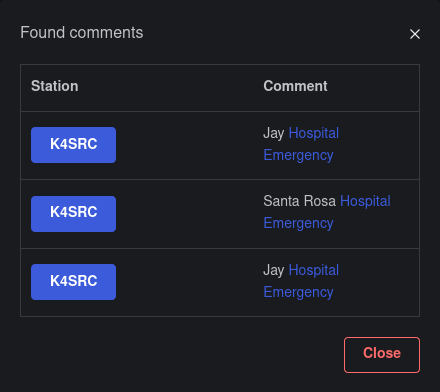
\includegraphics[width=0.5\textwidth]{Imagenes/Chapter_4/fts_output.png}
	\caption[Resultados de la búsqueda de <<emergency hospital>>.]{Resultados de la búsqueda de <<emergency hospital>> (elaboración propia).}
	\label{fig:postgres-fts}
\end{figure}

\noindent En el modal se muestra una tabla de dos columnas, la columna izquierda contiene un botón con el nombre de la estación y la columna derecha el contenido del mensaje.

\subsection{Station - Segunda pantalla}
Esta es la página que hace única a APRSINT. En esta página se muestra la información detallada de una estación APRS en concreto. Se puede llegar a esta pantalla desde la página principal haciendo clic en un marcador de una estación en el mapa, haciendo clic en una estación en la búsqueda en los mensajes o haciendo clic en un nodo del grafo de la página 3. La pantalla station está dividida en tres secciones.

\subsubsection*{Información de QRZ}
QRZ es una base de datos de radioaficionados que contiene información detallada sobre los radioaficionados de todo el mundo. Para acceder a la información disponible en la web de QRZ\footnote{\url{https://qrz.com}} es necesario tener una cuenta y estar registrado. QRZ cuenta con un servicio de API que permite acceder a la información de los radioaficionados de manera programática.

Para obtener la información de los radioaficionados se ha utilizado la librería requests de Python, que permite obtener la información necesaria de QRZ.

Con el fin de acelerar las consultas, se ha implementado una tabla en la base de datos para almacenar en caché las solicitudes, lo que disminuye la cantidad de consultas a una estación determinada si esta ya ha sido solicitada con anterioridad.

Este módulo es de los más complejos de la aplicación, pero a su vez de los más útiles, ya que permite al usuario obtener información muy detallada de una estación APRS en concreto y de la persona que está detrás. Algunos de los datos que se pueden obtener son:

\begin{itemize}
	\item Nombre de la persona registrada
	\item Fechas de registro y última actualización en la web
	\item Alias conocidos de la estación
	\item Dirección de la persona registrada (Como link a google maps)
	\item Fecha de nacimiento de la persona registrada
\end{itemize}

\subsubsection*{Información de posiciones}
Esta sección se compone de dos partes. En la parte superior se muestra un mapa con todas las posiciones reportadas por la estación, se muestra también la caja delimitadora de todas las posiciones.

En la parte inferior se muestran estadísticas de las posiciones reportadas por la estación como la frecuencia media de emisión, la primera y última emisión recibida y por cada mensaje emitido por la estación se muestra el número de repeticiones del mensaje y las URL (si existen) encontradas en los mensajes.

\subsubsection*{Información de mensajes}
Finalmente encontramos la sección de mensajes. En esta sección se muestra una tabla en la que se muestra la información de los mensajes emitidos por la estación. La tabla se compone de las siguientes columnas:
\begin{itemize}
	\item La fecha de emisión del mensaje.
	\item La latitud y longitud de la estación en el momento de la emisión.
	\item El país en el que se encontraba la estación en el momento de la emisión.
	\item La estación destino del mensaje.
	\item El \textit{path} es decir los \textit{Digipeaters} que han retransmitido el mensaje.
	\item El contenido del mensaje.
\end{itemize}

La tabla es interactiva y permite al usuario filtrar los mensajes por el intervalo de fechas que pretenda.

\subsection{Graph - Tercera pantalla}
Esta pantalla es la última de la web, en ella se muestra un grafo dirigido en el que los nodos son las estaciones y las aristas dirigidas, mensajes como se muestra en la \Cref{fig:graph}. El grafo es interactivo y permite hacer zoom, desplazarse y al posicionar el cursor encima de un nodo o arista aparecerá un recuadro ofreciendo información adicional. El color y tamaño de los nodos depende de la cantidad de mensajes que ha emitido o recibido la estación y de misma manera el color y tamaño de las aristas depende de la cantidad de mensajes que se han emitido o recibido desde la estación origen y destino.

\begin{figure}[h]
	\centering
	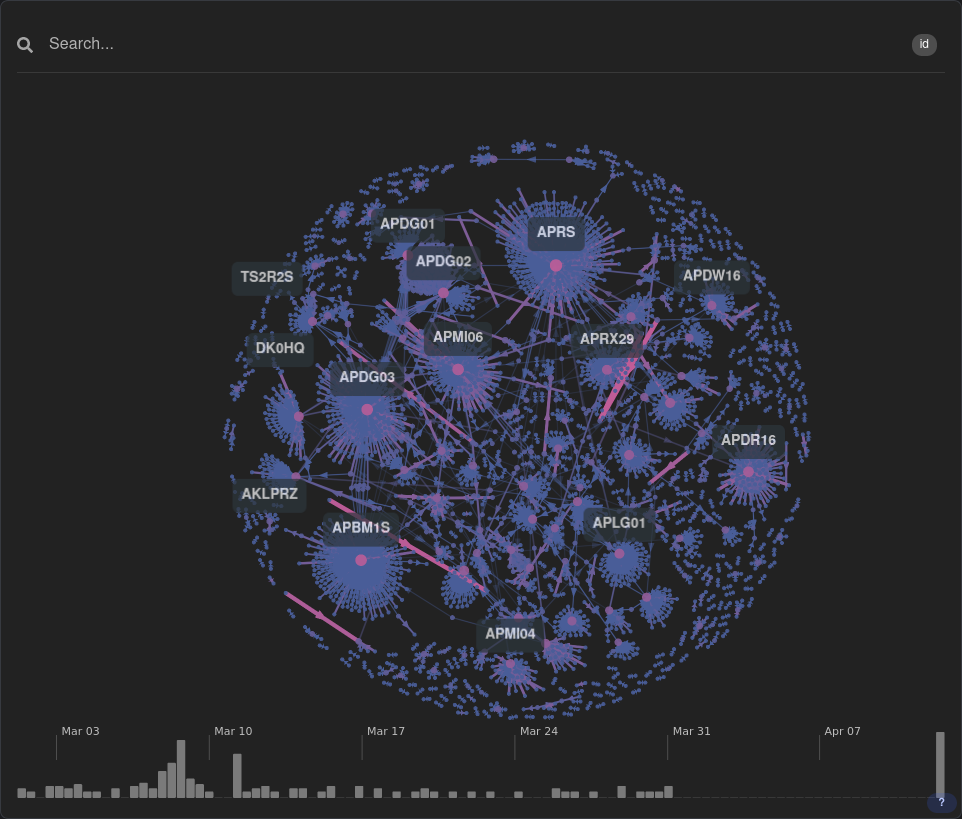
\includegraphics[width=0.85\textwidth]{Imagenes/Chapter_4/graph.png}
	\caption[Grafo de estaciones APRS.]{Grafo de estaciones APRS (elaboración propia).}
	\label{fig:graph}
\end{figure}

Las características que se buscaban en la solución final eran:

\begin{itemize}
	\item \textbf{Interactividad:} Se buscaba un grafo interactivo que permitiera al usuario explorar las relaciones entre las estaciones APRS.
	\item \textbf{Rendimiento:} Quizás la característica más importante, el grafo debía ser capaz de mostrar una gran cantidad de estaciones y conexiones sin afectar al rendimiento de la aplicación.
	\item \textbf{Personalización:} Se buscaba un grafo que permitiera personalizar la apariencia y el comportamiento de los nodos y aristas según las características de cada estación y mensaje.
\end{itemize}
Para alcanzar la solución final que se presenta ahora en la página, se han probado muchas opciones que se han ido descartando por diferentes motivos.
\subsubsection*{Alternativas probadas}
En un primer momento se intentó utilizar la librería \textbf{Networkx} de Python para la creación del grafo, sin embargo, se descartó debido a su rendimiento y a su falta de interactividad. Posteriormente se intentó utilizar la librería \textbf{Cytoscape} que es la solución por defecto que ofrece Dash, esta ofrece una gran cantidad de funcionalidades para la creación de grafos interactivos, sin embargo, se descartó de nuevo debido a su pobre rendimiento.

Una de las alternativas que también se probó fue la librería \textbf{Sigma JS} que ofrece una gran cantidad de funcionalidades y personalización para la creación de grafos interactivos. Esta librería cuenta con una funcionalidad interesante \textit{forceAtlas2} que permite calcular mediante una simulación de fuerzas la posición de los nodos y aristas en el grafo. Sin embargo, de nuevo se descartó debido a su rendimiento con una gran cantidad de nodos y aristas.

Finalmente se optó por la librería \textbf{Cosmograph JS}. Cosmograph utiliza la librería \textit{Cosmos} de cálculo de posiciones mediante la GPU y por tanto puede manejar un gran número de nodos y aristas.

\subsubsection*{El Grafo}
El problema principal con Cosmograph ha sido la falta de documentación debido a que es bastante nueva y la dificultad de integrarla con Dash. Esta librería está publicada en NPM (el repositorio de librerias de JavaScript) y se ha tenido que utilizar bundle.js para convertir el código de JavaScript en un solo fichero que se pueda importar en Dash. Ha sido necesario modificar ligeramente la librería para terminar de integrarla con Dash.

Se han utilizado tres componentes de Cosmograph JS para la creación del grafo, el componente \textit{Cosmograph} que crea el grafo, el componente \textit{CosmographSearch} que permite mediante una barra de búsqueda encontrar una estación y el componente \textit{CosmographTimeline} que permite filtrar el grafo por rango de fechas.

Para mejorar el rendimiento general de la web se ha utilizado la técnica de lazy-loading, que consiste en cargar los componentes del grafo solo cuando el usuario presiona el botón \textit{Load graph}. En el momento que el usuario presiona el botón, se activa un callback de cliente de Dash. El callback primero lee los datos del grafo de un fichero CSV que se actualiza diariamente mediante Apache Airflow. Posteriormente se crean los nodos y las aristas y se inicializa el grafo, la barra de búsqueda y la barra de tiempo. Seguidamente se establecen los parámetros de la simulación de fuerzas y se inicia la simulación. Por último se establecen las propiedades visuales y funcionales de los nodos y aristas.

Cuando el usuario arrastra el cursor sobre un nodo, se muestra un recuadro con el nombre de la estación. Cuando el usuario hace clic en un nodo, se le redirige a la página \textbf{station} de la estación seleccionada.

\section{Orquestación}

En esta sección se describe con detalle la metodología de orquestación de tareas y flujos de trabajo de la aplicación que se han ido comentando a lo largo del capítulo.

\subsection{Supervisord}
Supervisord es un sistema de control de procesos para sistemas operativos tipo Unix, diseñado para iniciar, detener y gestionar procesos de manera sencilla y robusta.

Se ha utilizado Supervisord como gestor de procesos para ejecutar en modo demonio como se ha mencionado previamente el sistema de recepción de paquetes APRS. Se ha establecido en la configuración de Supervisord que el sistema de recepción de paquetes se ejecute en el arranque del sistema y siempre después de que la interfaz de red esté disponible. En caso de fallo del sistema de recepción, Supervisord reiniciará el sistema y registrará la causa del fallo.

\section{Apache Airflow}
Apache Airflow es una plataforma de orquestación de tareas y flujos de trabajo. Es similar a Cron de Unix, pero permite al usuario una mayor personalización y un mayor control sobre las tareas que controla. La unidad de ejecución en Apache Airflow es el DAG (Directed Acyclic Graph). Las tareas se definen en archivos individuales y al igual que en otros sistemas se pueden definir dependencias entre tareas.

Apache Airflow se ha utilizado para orquestar todas las tareas que permiten que APRSINT funcione correctamente se presenta en la Tabla \ref{tab:airflow-sched} la lista de los DAG's que se ejecutan diariamente.

\begin{table}[htbp]
	\centering
	\begin{tabular}{|c|c|m{5.5cm}|}
		\hline
		\textbf{Hora de ejecución} & \textbf{DAG} & \textbf{Descripción} \\
		\hline
		3:00 am & upload\_files & Sube todos los archivos al S3 aprsinput \\
		\hline
		5:00 am & download\_files & Descarga todos los archivos a la carpeta local \\
		\hline
		7:00 am  & insert\_database & Inserta todos los mensajes en la BBDD \\
		\hline
		9:00 am & cache\_data & Precalcula en archivos los datos para la web \\
		\hline
	\end{tabular}
	\caption{Esquema de orquestación con Apache Airflow.}
	\label{tab:airflow-sched}
\end{table}

Por defecto Apache Airflow utiliza una base de datos SQLite para almacenar los metadatos de las tareas y los flujos de trabajo. Sin embargo, para este proyecto se ha optado por utilizar una base de datos PostgreSQL para almacenar los metadatos de Apache Airflow. Esto se ha hecho para mejorar la escalabilidad y sobre todo la fiabilidad del sistema.

Se ha creado también un usuario en la base de datos de PostgreSQL con permisos de lectura y escritura para Apache Airflow. Se ha configurado Apache Airflow para que utilice esta base de datos y este usuario en el archivo de configuración de Apache Airflow.

Otra configuración importante que se ha realizado en Apache Airflow es el cambio del ejecutor por defecto de SequentialExecutor a LocalExecutor. El ejecutor por defecto de Apache Airflow es SequentialExecutor, que ejecuta las tareas de manera secuencial en un solo hilo. Sin embargo, no se recomienda el uso de este ejecutor por lo que para mejorar el rendimiento y la escalabilidad del sistema se ha optado por utilizar LocalExecutor, que ejecuta las tareas de manera paralela en varios hilos.

Se presenta en la \Cref{fig:airflow-dashboard} la interfaz de Apache Airflow con los DAG's que se ejecutan diariamente.

\begin{figure}[h]
	\centering
	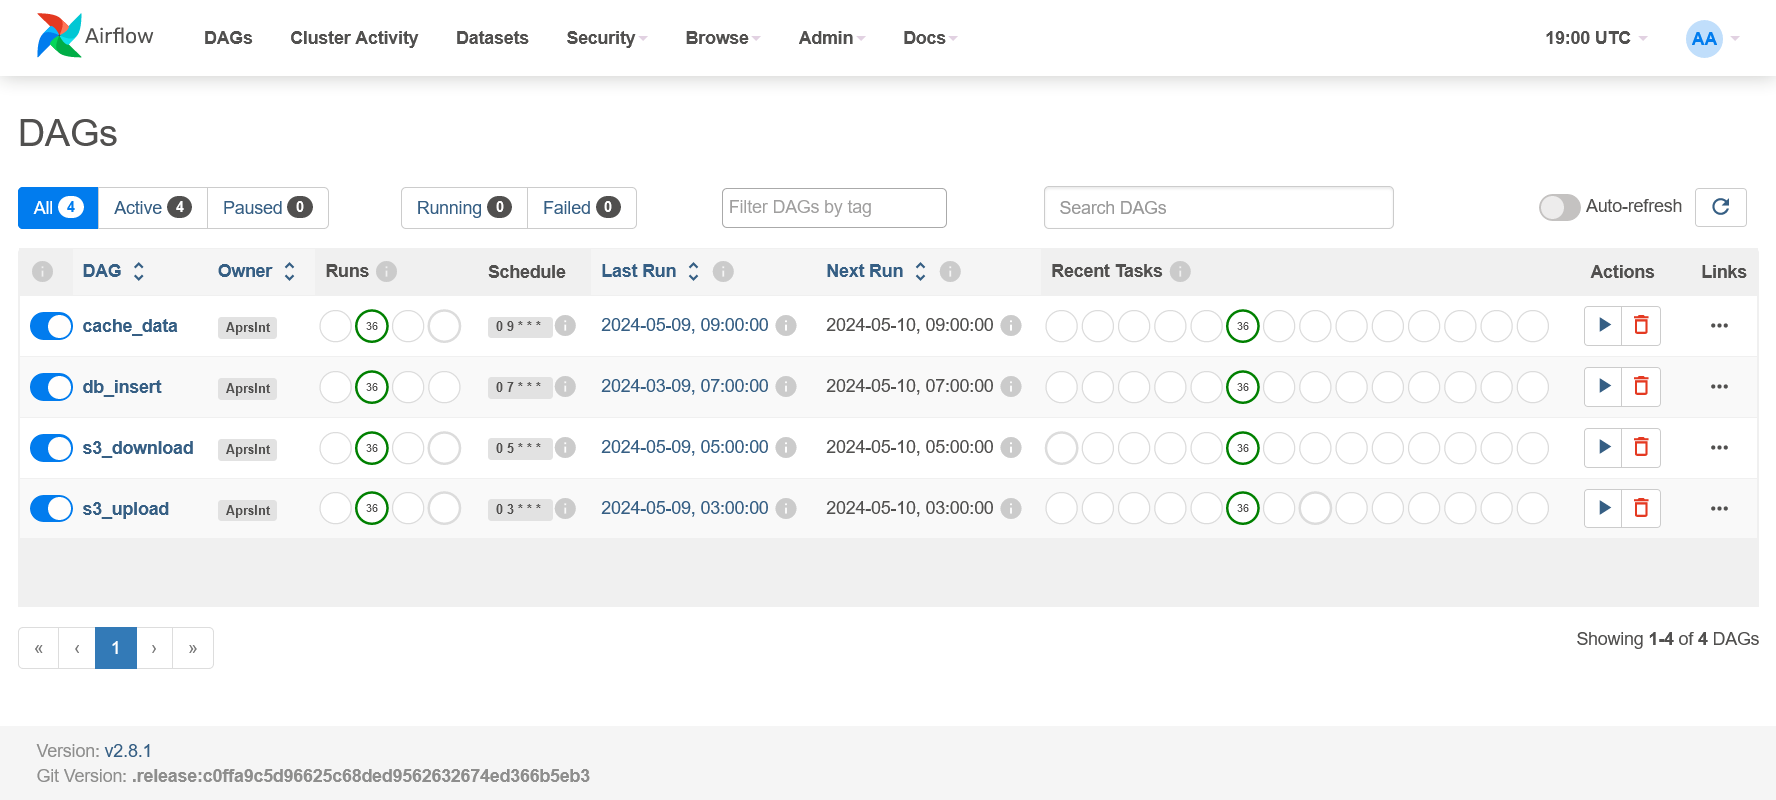
\includegraphics[width=1\textwidth]{Imagenes/Chapter_4/airflow_dashboard.png}
	\caption[Interfaz de Apache Airflow.]{Interfaz de Apache Airflow (elaboración propia).}
	\label{fig:airflow-dashboard}
\end{figure}

\section{Alojamiento}
Para alojar tanto la aplicación web como el sistema de recepción de paquetes y la base de datos de APRSINT se ha optado por utilizar una Raspberry Pi 4 conectada a un internet residencial.

Para evitar los problemas que suponen las direcciones dinámicas se ha decidido por utilizar el servicio de DNS dinámico de no-ip que permite asignar un nombre de dominio a una dirección ip dinámica. Este sistema se ha configurado en el router de modo que cuando la dirección ip cambia, el router notifica a no-ip y este actualiza el registro DNS asociado a la ip antigua por la nueva dirección.

Se ha configurado también la redirección de puertos en el router para permitir el acceso a la Raspberry Pi desde el exterior. Los servidores que se encuentran actualmente en la Raspberry Pi son:
\begin{itemize}
	\item \textbf{Servidor Web:} Se ha configurado un servidor web Nginx para servir la aplicación web de APRSINT.
	\item \textbf{Base de Datos:} Se ha configurado un servidor PostgreSQL para almacenar los metadatos de Apache Airflow y los datos de los mensajes APRS.
	\item \textbf{Apache Airflow:} Se ha configurado un servidor Apache Airflow para orquestar las tareas y flujos de trabajo de APRSINT.
	\item \textbf{Servidor SSH:} Se ha configurado un servidor SSH para permitir el acceso remoto a la Raspberry Pi y realizar todo el desarrollo.
\end{itemize}

\subsection{Servidor Web}

En esta sección se describen las tecnologías y la arquitectura del servidor web que aloja la aplicación web de APRSINT. La aplicación utiliza el \textit{framework} Flask como backend web, junto con Gunicorn como servidor web WSGI y Nginx como reverse proxy.

\subsubsection*{Flask}

Flask es un \textit{framework} web ligero para Python que proporciona herramientas para crear aplicaciones web de forma rápida y sencilla. En esta aplicación, Flask se utiliza como el \textit{framework} backend para la aplicación de Dash. Proporciona las rutas y la lógica de negocio necesarias para la aplicación.

\subsubsection*{Gunicorn}

Gunicorn es un servidor HTTP WSGI (Web Server Gateway Interface) para Python. Se utiliza para servir la aplicación Flask de forma eficiente y escalable. Gunicorn gestiona múltiples procesos de forma paralela, lo que mejora el rendimiento de la aplicación.

Para APRSINT se ha configurado Gunicorn para ejecutar la aplicación Flask en modo demonio y con 4 procesos de trabajo. Gunicorn crea un socket UNIX en el que escucha las solicitudes HTTP y las reenvía a la aplicación Flask para su procesamiento.

\subsubsection*{Nginx}

Nginx es un servidor web de código abierto que en este caso se ha utilizado como proxy inverso. Actúa como intermediario entre los clientes y el servidor Flask / Gunicorn. Nginx se encarga de recibir las solicitudes HTTP, dirigirlas al servidor Gunicorn y devolver las respuestas a los clientes. Nginx maneja tareas como el balanceo de carga, el almacenamiento en caché la compresión de archivos y la seguridad. Se ha configurado Nginx para servir la aplicación web de APRSINT en el puerto 80 (local).

El diagrama de la arquitectura del servidor web se muestra en la \Cref{fig:web-server}. Como se puede observar, la solicitud HTTP del cliente pasa a través de Nginx, que actúa como un proxy inverso y la reenvía a Gunicorn, donde se ejecuta la aplicación Flask. Una vez que Flask procesa la solicitud, la respuesta se envía de vuelta al cliente a través de Nginx.

\begin{figure}[h]
	\centering
	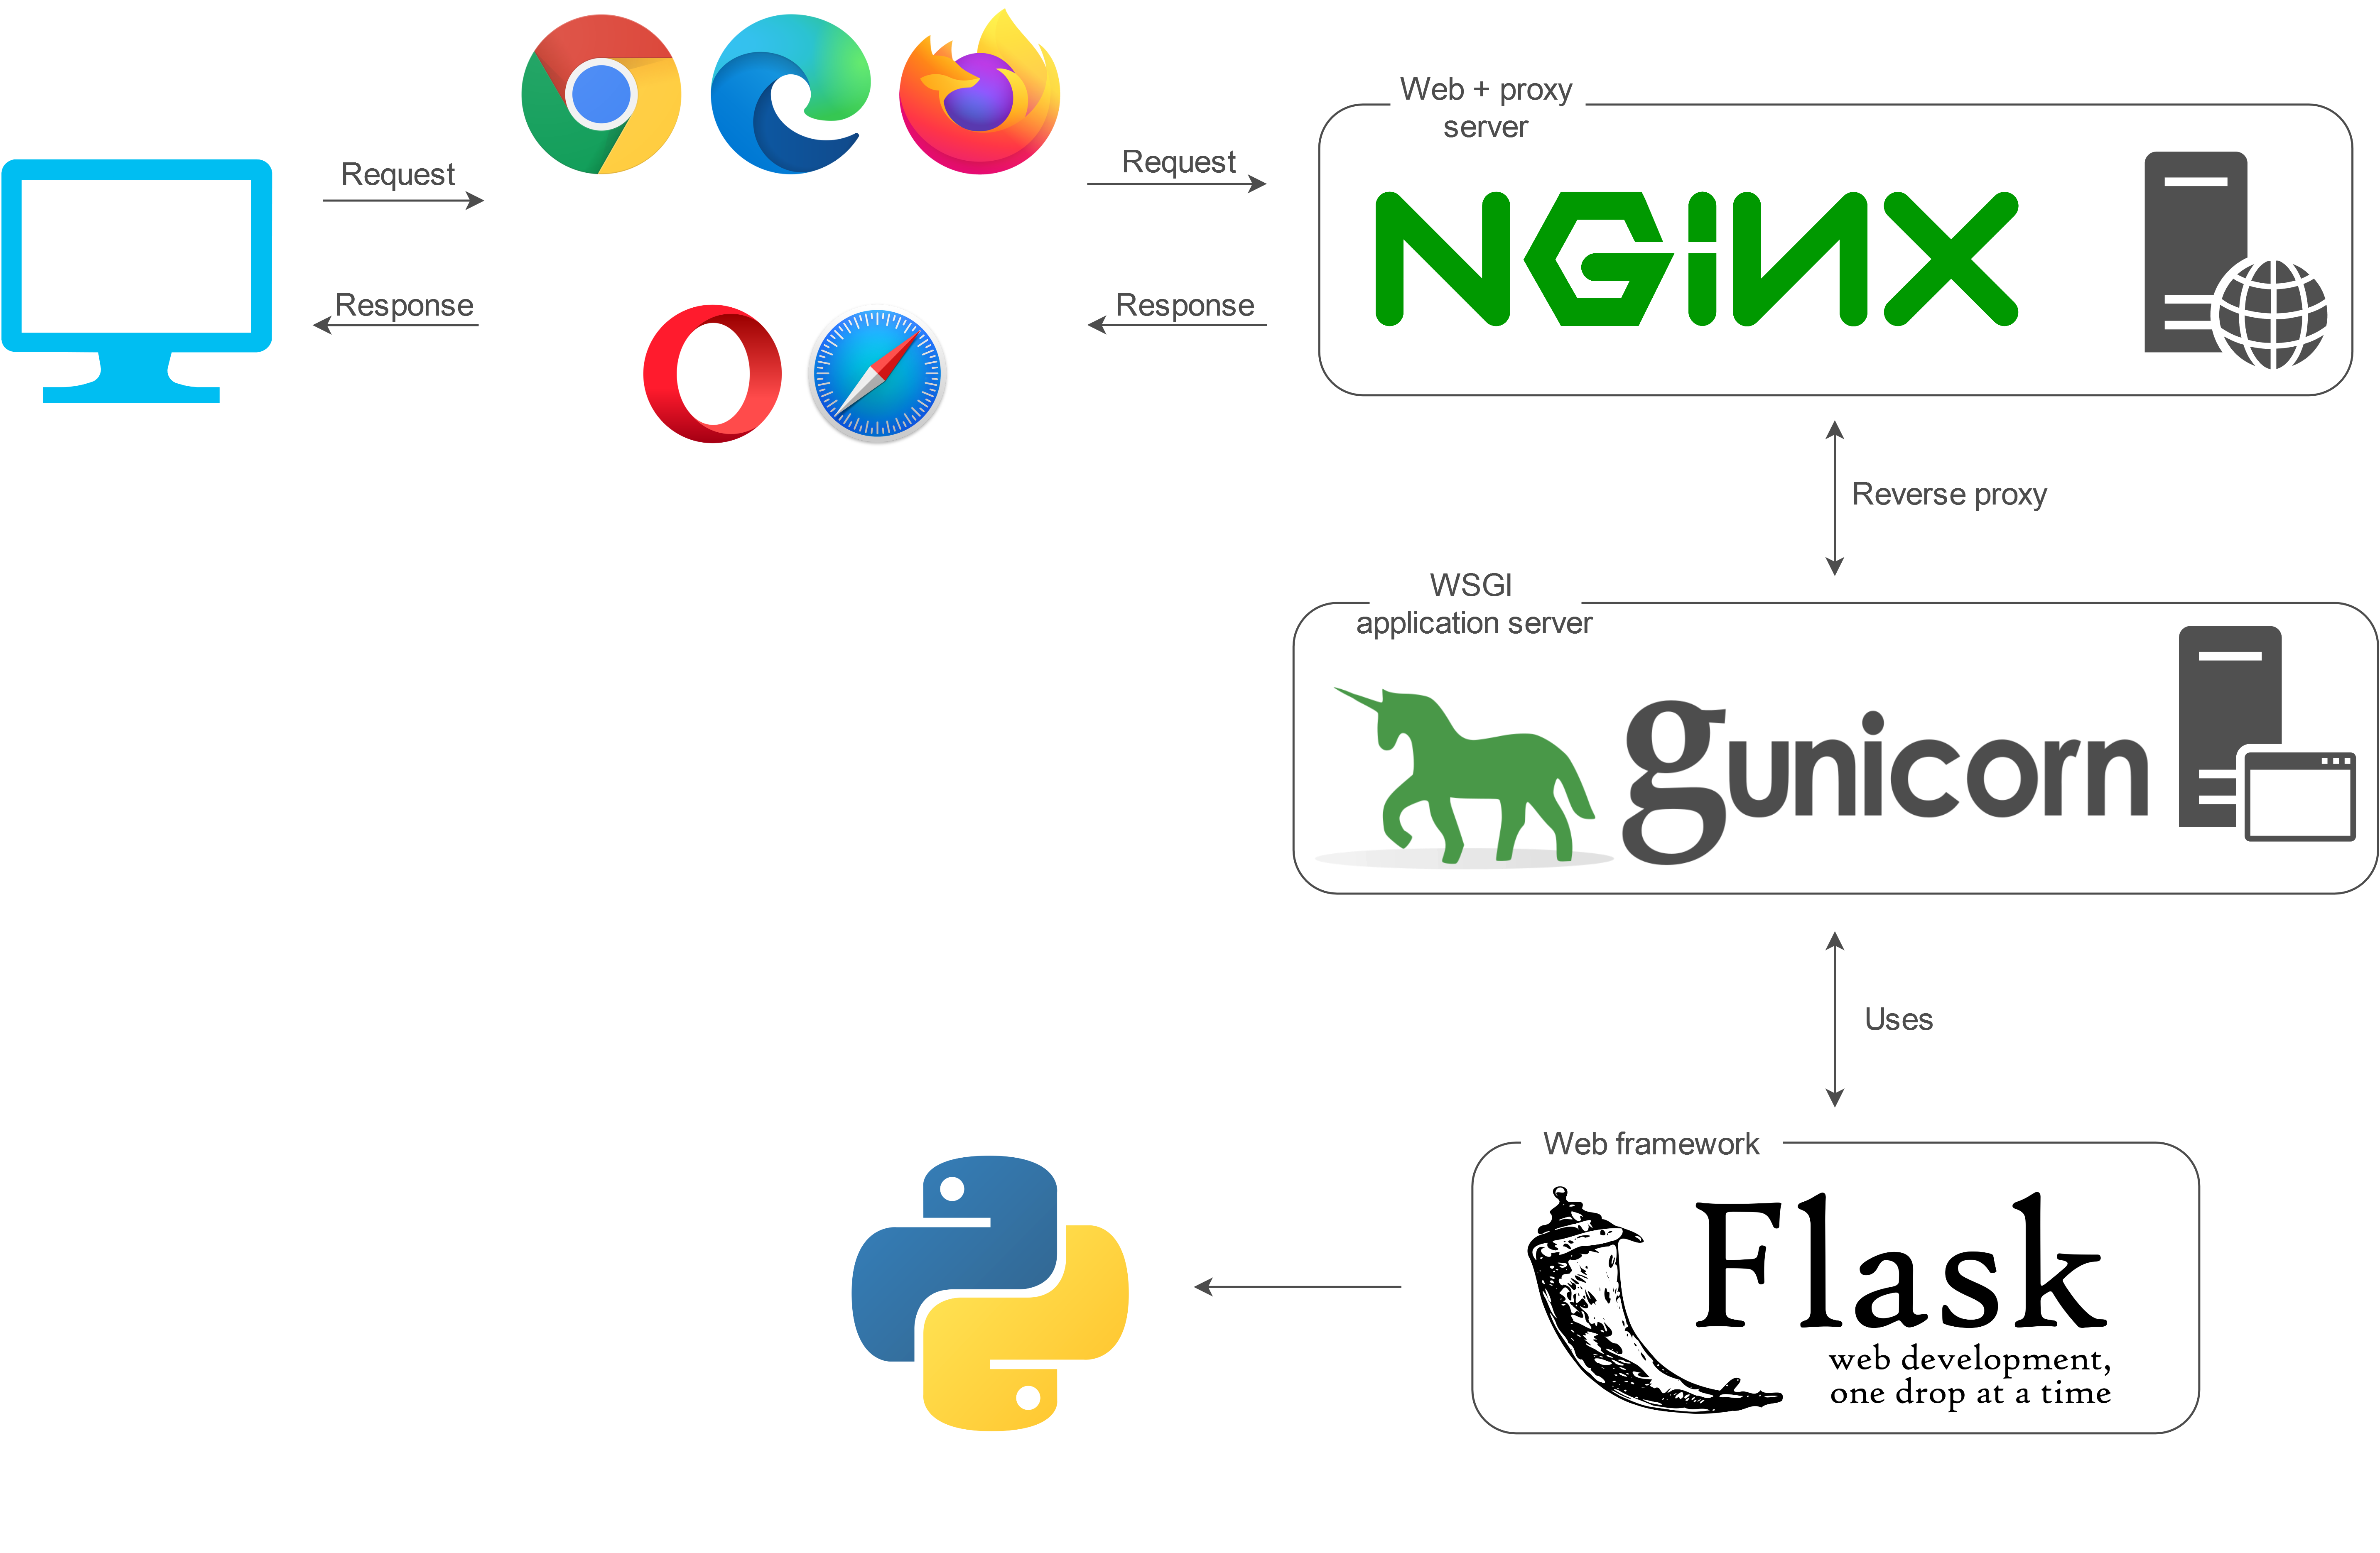
\includegraphics[width=0.9\textwidth]{Imagenes/Chapter_4/web_server.png}
	\caption[Arquitectura del servidor web de APRSINT.]{Arquitectura del servidor web de APRSINT (elaboración propia).}
	\label{fig:web-server}
\end{figure}

\subsubsection*{Flujo de una petición HTTP}

A continuación se describe cómo se maneja una solicitud HTTP desde se recibe en Nginx hasta que se envía la respuesta de vuelta al cliente. A continuación se detalla el proceso paso a paso:

\begin{enumerate}
	\item Un usuario busca en su navegador la aplicación web de APRSINT.
	\item La solicitud llega al servidor Nginx, que actúa como el servidor frontal.
	\item Nginx examina la solicitud y determina que está destinada a la aplicación Dash, por lo que la reenvía al servidor Gunicorn.
	\item Gunicorn recibe la solicitud y la asigna a uno de sus 4 procesos de Flask para su procesamiento.
	\item La aplicación Flask ejecuta la lógica correspondiente a la solicitud, que incluyen el acceso a la base de datos, y la generación del contenido de la página.
	\item Una vez que la lógica de la aplicación Flask se ha completado, se genera una respuesta.
	\item La respuesta se envía de vuelta a Gunicorn, que la reenvía a Nginx.
	\item Nginx recibe la respuesta y la devuelve al cliente que realizó la solicitud original.
\end{enumerate}

Este proceso asegura que las solicitudes sean manejadas de manera eficiente y escalable, garantizando una experiencia de navegación más fluida.

\subsection{Protección ante ataques}

En el desarrollo de la aplicación, se ha priorizado la seguridad como un aspecto fundamental. Se han implementado varias medidas para proteger el sistema contra posibles ataques externos e internos. A continuación, se detallan algunas de las estrategias de seguridad utilizadas:

\begin{itemize}
    \item \textbf{Uso del protocolo SSH:} Se ha optado por utilizar exclusivamente el protocolo SSH (Secure Shell) para la administración y desarrollo remoto de la Raspberry Pi. El SSH proporciona una conexión segura y cifrada, lo que reduce el riesgo de interceptación de datos sensibles durante la comunicación.
    
    \item \textbf{Creación de un usuario no root:} Se ha creado un usuario no root con privilegios limitados para las operaciones diarias. Esto ayuda a mitigar el impacto de posibles vulnerabilidades en el sistema, ya que el acceso de usuario se limita a las funciones esenciales.
    
    \item \textbf{Cambio del puerto SSH por defecto:} Como medida adicional de seguridad, se ha cambiado el puerto predeterminado del servicio SSH. Esto dificulta los intentos de acceso no autorizado, ya que los atacantes suelen escanear los puertos estándar en busca de vulnerabilidades.
    
    \item \textbf{Desactivación del acceso por contraseña:} Se ha desactivado el acceso por contraseña al servidor SSH, lo que significa que los usuarios deben autenticarse mediante claves SSH. Este enfoque reduce el riesgo de ataques de fuerza bruta dirigidos a contraseñas débiles.
    
    \item \textbf{Instalación de fail2ban:} Se ha instalado y configurado \textbf{fail2ban}, una herramienta de prevención de intrusiones que monitoriza los registros del sistema en busca de intentos de acceso fallidos. Fail2ban bloquea automáticamente las direcciones ip de los atacantes después de un número especificado de intentos fallidos, lo que ayuda a proteger contra ataques de fuerza bruta.
    
    \item \textbf{Configuración de un firewall UFW:} Se ha configurado el firewall ``Uncomplicated Firewall'' (UFW) para controlar el tráfico de red entrante y saliente. El firewall UFW bloquea el acceso a los puertos no utilizados y permite especificar reglas de acceso para servicios específicos, lo que ayuda a prevenir intrusiones no autorizadas.
    
	\item \textbf{Actualizaciones regularer del sistema:} Se ha establecido un \textit{cronjob} para que actualice el sistema operativo y las aplicaciones instaladas regularmente. Las actualizaciones de seguridad y los parches de \textit{software} son esenciales para proteger el sistema contra vulnerabilidades conocidas.
\end{itemize}

\noindent Mediante estas estrategias, se pretende minimizar los riesgos de seguridad y proteger la integridad y la confidencialidad de los datos de la aplicación.

\section{Casos de uso}

En esta sección se describen los casos de uso de la aplicación web de APRSINT, incluyendo los actores, las funcionalidades y los escenarios de uso.

Se ha identificado a dos actores principales en la aplicación web de APRSINT:
\begin{itemize}
	\item \textbf{Investigador de OSINT:} Este actor utilizará funciones avanzadas de filtrado para analizar y extraer inteligencia de los datos APRS. El investigador de OSINT busca obtener información detallada y procesable a partir de los mensajes transmitidos, utilizando herramientas sofisticadas para explorar patrones, tendencias y relaciones en los datos.
	\item \textbf{Radioaficionados curiosos:} Estos actores son entusiastas de la radioafición que visitarán la aplicación web de APRSINT principalmente por curiosidad y para explorar el mundo de APRS de una manera más interactiva y visual. Aunque pueden no tener experiencia en análisis avanzado de datos, están interesados en descubrir nuevas estaciones, rutas de seguimiento y eventos en tiempo real utilizando la plataforma.
\end{itemize}

\noindent Se han identificado las siguientes funcionalidades y escenarios de uso para la aplicación web de APRSINT:
\begin{itemize}
	\item \textbf{Visualización de estaciones APRS:} Los usuarios de la aplicación pueden visualizar las estaciones APRS en un mapa interactivo, proporcionando una representación geográfica del panorama APRS.
	\item \textbf{Filtrado de estaciones APRS:} Permite a los usuarios filtrar las estaciones APRS según criterios específicos, como rango de fechas, país, contenido del mensaje, tipo de estación y SSID, para obtener información relevante.

	\item \textbf{Búsqueda de mensajes:} Se pueden buscar mensajes emitidos por las estaciones que contengan una palabra o frase específica, facilitando la localización de información relevante en la red APRS.

	\item \textbf{Visualización de información detallada de una estación APRS:} Esta funcionalidad permite acceder a información detallada de una estación APRS en particular, incluyendo datos de identificación, posiciones reportadas y mensajes emitidos, para un análisis más profundo.

	\item \textbf{Visualización del grafo de estaciones APRS:} Los usuarios pueden visualizar un grafo que representa las conexiones entre las estaciones APRS, proporcionando una visualización clara de la estructura de la red APRS.

	\item \textbf{Exploración del grafo de estaciones APRS:} Permite la exploración del grafo de estaciones APRS interactuando con los nodos y enlaces, obteniendo información adicional sobre las relaciones entre las estaciones.

	\item \textbf{Descarga de datos:} Facilita la descarga de los datos de las estaciones APRS en formato CSV, facilitando su análisis fuera de la plataforma APRSINT.

\end{itemize}

\noindent Estas son las funcionalidades y escenarios de uso que se han diseñado para satisfacer las necesidades de los dos actores y proporcionar una experiencia completa en APRSINT.